% use paper, or submit
% use 11 pt (preferred), 12 pt, or 10 pt only

%\documentclass[letterpaper, preprint, paper,11pt]{AAS}	% for preprint proceedings
%\documentclass[letterpaper, paper,11pt]{AAS}		% for final proceedings (20-page limit)
%\documentclass[letterpaper, paper,12pt]{AAS}		% for final proceedings (20-page limit)
\documentclass[letterpaper, paper,10pt]{AAS}		% for final proceedings (20-page limit)
%\documentclass[letterpaper, submit]{AAS}			% to submit to JAS

\usepackage{bm}
\usepackage{amsmath}
\usepackage{subfigure}
%\usepackage[notref,notcite]{showkeys}  % use this to temporarily show labels
\usepackage[colorlinks=true, pdfstartview=FitV, linkcolor=black, citecolor= black, urlcolor= black]{hyperref}
\usepackage{overcite}
\usepackage{footnpag}	
\usepackage{amssymb,url}
\usepackage{graphicx,subfigure,tikz,graphicx}
\usepackage{color}
\usepackage{csquotes}		      	% make footnote symbols restart on each page
\usepackage{amssymb,amsmath,amsthm,times,graphicx,subfigure,tabularx,booktabs,colortbl,multirow,threeparttable}

\newcommand{\hilight}[1]{\colorbox{green}{#1}}
\newcommand{\argmax}{\operatornamewithlimits{argmax}}
\newcommand{\expm}{\ensuremath{\mathrm{expm}}}
\newcommand{\diag}{\mathop{\mathrm{diag}}\nolimits}
\newcommand{\norm}[1]{\ensuremath{\left\| #1 \right\|}}
\newcommand{\bracket}[1]{\ensuremath{\left[ #1 \right]}}
\newcommand{\braces}[1]{\ensuremath{\left\{ #1 \right\}}}
\newcommand{\parenth}[1]{\ensuremath{\left( #1 \right)}}
\newcommand{\pair}[1]{\ensuremath{\langle #1 \rangle}}
\newcommand{\met}[1]{\ensuremath{\langle\langle #1 \rangle\rangle}}
\newcommand{\refeqn}[1]{(\ref{eqn:#1})}
\newcommand{\reffig}[1]{Fig. \ref{fig:#1}}
\newcommand{\tr}[1]{\mathrm{tr}\ensuremath{\negthickspace\bracket{#1}}}
\newcommand{\trs}[1]{\mathrm{tr}\ensuremath{[#1]}}
\newcommand{\ave}[1]{\mathrm{E}\ensuremath{[#1]}}
\newcommand{\deriv}[2]{\ensuremath{\frac{\partial #1}{\partial #2}}}
\newcommand{\SO}{\ensuremath{\mathsf{SO(3)}}}
\newcommand{\T}{\ensuremath{\mathsf{T}}}
\renewcommand{\L}{\ensuremath{\mathsf{L}}}
\newcommand{\so}{\ensuremath{\mathfrak{so}(3)}}
\newcommand{\SE}{\ensuremath{\mathsf{SE(3)}}}
\newcommand{\se}{\ensuremath{\mathfrak{se}(3)}}
\renewcommand{\Re}{\ensuremath{\mathbb{R}}}
\newcommand{\aSE}[2]{\ensuremath{\begin{bmatrix}#1&#2\\0&1\end{bmatrix}}}
\newcommand{\ase}[2]{\ensuremath{\begin{bmatrix}#1&#2\\0&0\end{bmatrix}}}
\newcommand{\D}{\ensuremath{\mathbf{D}}}
\renewcommand{\d}{\ensuremath{\mathfrak{d}}}
\newcommand{\Sph}{\ensuremath{\mathsf{S}}}
\renewcommand{\S}{\Sph}
\newcommand{\J}{\ensuremath{\mathbf{J}}}
\newcommand{\Ad}{\ensuremath{\mathrm{Ad}}}
\newcommand{\intp}{\ensuremath{\mathbf{i}}}
\newcommand{\extd}{\ensuremath{\mathbf{d}}}
\newcommand{\hor}{\ensuremath{\mathrm{hor}}}
\newcommand{\ver}{\ensuremath{\mathrm{ver}}}
\newcommand{\dyn}{\ensuremath{\mathrm{dyn}}}
\newcommand{\geo}{\ensuremath{\mathrm{geo}}}
\newcommand{\Q}{\ensuremath{\mathsf{Q}}}
\newcommand{\G}{\ensuremath{\mathsf{G}}}
\newcommand{\g}{\ensuremath{\mathfrak{g}}}
\newcommand{\Hess}{\ensuremath{\mathrm{Hess}}}
\newcommand{\Ibd}{\ensuremath{\mathbf{1}_{bd}}}
\newcommand\circled[1]{%
  \tikz[baseline=(C.base)]\node[draw,circle,inner sep=0.5pt](C) {#1};\!
}




\PaperNumber{27-432}



\begin{document}

\title{Minimum Uncertainty JPDA Filter and Coalescence Avoidance Performance Evaluations}

\author{Evan Kaufman\thanks{Doctoral Student, Mechanical and Aerospace Engineering, George Washington University, 801 22nd St NW, Washington, DC 20052, Email: evankaufman@gwu.edu.},  
T. Alan Lovell\thanks{Research Aerospace Engineer, Air Force Research Laboratory, Space Vehicles Directorate, Kirtland AFB, NM.},
\ and Taeyoung Lee\thanks{Assistant Professor, Mechanical and Aerospace Engineering, George Washington University, 801 22nd St NW, Washington, DC 20052, Tel: 202-994-8710, Email: tylee@gwu.edu.}
\thanks{This research has been supported in part by NSF under the grants CMMI-1243000 (transferred from 1029551), CMMI-1335008, and CNS-1337722.}
}


\maketitle{} 		


\begin{abstract}
Two variations of the joint probabilistic data association filter (JPDAF) are derived and simulated extensively in this paper.
First, an analytic solution for an optimal gain that minimizes posterior estimate uncertainty is derived, referred to as the minimum uncertainty JPDAF (MUJPDAF).
Second, the coalescence-avoiding optimal JPDAF (C-JPDAF) is derived, which removes coalescence by minimizing a weighted sum of the posterior uncertainty and a measure of similarity between estimated probability densities.
Both novel algorithms are tested in much further depth than any prior work to show how the algorithms perform in various scenarios.
In particular, the MUJPDAF more accurately tracks objects than the conventional JPDAF in all simulated cases.
When coalescence degrades the estimates at too great of a level, and the C-JPDAF is often superior at removing coalescence when its parameters are properly tuned.
\end{abstract}


\section{Introduction}

Data association has been extensively studied with various applications in estimation when measurements are not necessarily originating from a single object.
We consider applications wherein multiple objects of interest enter the field of view of a sensor; however, the measurement origins are unknown.
To properly track these objects, we require estimation techniques that associate objects with measurements.
When the objects are in very close proximity, the association uncertainties grow, and an effective algorithm is necessary to maintain close estimations of the objects~\cite{KauLovLee14}.

A variety of data association techniques are considered for close-proximity trajectories with varying performance.
Multiple hypothesis tracking (MHT) and probability hypothesis density (PHD) techniques involve a high computational load, especially when objects are in close proximity, making real-time implementation more difficult~\cite{MHT1,PHD1,PHD2}.
Many other techniques are based on the Kalman filter (KF) or the extended KF (EKF), which provide a framework for recursive data association techniques for easier real-time implementation.
There are two popular strategies among recursive approaches, namely \emph{hard decisions} and \emph{soft decisions}~\cite{JPDAF1}.
A hard decision is when estimates are fully associated with measurements according to some metric between the estimates and the measurements.
For example, a common heuristic approach is known as the nearest neighbor filter (NNF), which uses the Mahalanobis distance between each measurement and the predicted measurements of each potential object to determine likely associations.
The measurement with the smallest Mahalanobis distance is considered as the correct one~\cite{NN2}.
However, when estimates are in close proximity, there is a high likelihood of making incorrect associations, which may be detrimental to the estimated states, so this technique is avoided in the analysis of this paper.

Alternatively with a soft decision technique such as the joint probabilistic data association filter (JPDAF), measurements are shared among the estimates. With the JPDAF, the likelihoods of association between measurements and estimates serve as weighting factors inside the measurement update portion of the filtering~\cite{JPDAF1,TrackDataAssoc}.
The JPDAF is particularly advantageous in multi-object scenarios because when objects share measurements, the soft decisions prevent loss of information, which occurs with hard decision approaches.
%The a posteriori uncertainties of the estimates are changed because of an additional term representing the spread in the innovations; the Kalman gain serves as a close estimate to an optimal gain in the sense that in nearly minimizes this a posteriori gain as derived by the linearized equations of the JPDAF.
The JPDAF is based on the Kalman gain, which minimizes the posterior uncertainty of individual tracks.
However, the Kalman gain is not guaranteed to \emph{exactly} minimize the posterior uncertainties as they are defined for the JPDAF.
In fact, the JPDAF is applied to multi-target tracking applications widely with the incorrect assumption that the Kalman gain yields an optimal estimator.
%The unnecessarily large uncertainty of the suboptimal Kalman gain serves as motivation to derive an optimal gain that minimizes the a posteriori uncertainty of the linearized JPDAF equations.

In this paper, we show the derivation of the optimal estimation gain that minimizes the magnitude of the posterior covariance matrix that maintains the framework of the JPDAF.
The resulting minimum uncertainty JPDAF is referred to as the MUJPDAF, where this new algorithm is neither more complicated nor more computationally expensive than the conventional JPDAF.
We show that decreasing estimate uncertainty to its minimum value increases the confidence of associating measurements to estimates through various numerical examples.

Additionally, this paper deals with cases when neighboring objects share measurements, where the estimates are subject to coalescence.
Most techniques to avoid track coalescence involve pruning the tracks, or designing a set of rules that limit the possible outcomes to likely scenarios. These rules typically involve exact nearest neighbor probabilistic data association (ENNPDA), which applies a strong decision to the most likely associated estimate. Pruning algorithms incorporate the ENNPDA algorithm because  estimates do not share measurements, making it insensitive to track coalescence~\cite{Coal1}.
For example in~\cite{Fitzgerald}, the algorithm involves a set of rules to prune the tracks that share measurements.
The algorithm considers the possible combinations of estimate-to-measurement associations over a time window and applies a logic that assigns estimates to likely scenarios; only a small set of possible scenarios are considered and lower likelihood scenarios are deleted~\cite{Coal_d,Coal_e,Coal_c}.
However, track pruning assumes that low likelihood association scenarios are incorrect, which is not necessarily true.
Furthermore, removing the weighting scheme of the JPDAF causes the estimates to lose information.

Therefore, we propose a new coalescence-avoiding optimal JPDAF, referred to as the C-JPDAF, which is a systematic approach to remove coalescence by minimizing the weighted sum of the uncertainty and a similarity index between estimates.
The prior work from~\cite{KauLovLee14} covers the concept in simple cases, assuming that only two objects are considered with a single measurement at each time step, and that the state and measurement are very similar.
These assumptions are unrealistic in most scenarios.
Therefore, we generalize the C-JPDAF algorithm in this paper to handle (i) any number of objects and measurements, (ii) missed detections and measurements originating from extraneous clutter, and (iii) measurements with a much different interpretation than just the object states.

This paper serves two major purposes:
first, it provides a thorough derivation and relevant proofs for the MUJPDAF and C-JPDAF for a generalized system of estimates where measurement origins are uncertain.
Second, the algorithms undergo extensive numerical simulations with orbiting satellites that provide insight into the effects of various parameters on the algorithms.

% Cut from the abstract (summary of what is above)
%This paper analyzes variations on a popular approach known as the joint probabilistic data association filter (JPDAF).
%The JPDAF is advantageous because of its low computational requirements for real time implementation and its heavily tested successful data association with missed detections and measuring extraneous clutter.
%The JPDAF is based on the Kalman gain, which minimizes the posterior uncertainty of individual tracks.
%However, the Kalman gain is not guaranteed to \emph{exactly} minimize the posterior uncertainties of the JPDAF.
%Therefore, a minimum uncertainty JPDAF (MUJPDAF) is derived, which provides an analytic solution to a gain that minimizes the posterior uncertainty~\cite{KauLovLee15}.
%This algorithm shows significant improvements by decreasing estimate uncertainties and coalescence when compared with the JPDAF.
%
%Additionally, when measurements are shared among the estimates, the measurement updates tend to coalesce the estimates.
%A generalized coalescence-avoiding optimal JPDAF is proposed, where a similarity measure is included in the cost function to solve for a gain matrix inside the filter~\cite{KauLovLee15}.
%
%However, the MUJPDAF and C-JPDAF are only simulated in a few scenarios.
%This paper shows the performance of the JPDAF, MUJPDAF, and C-JPDAF in various cases with orbiting satellites where associating measurements to estimates is a challenge.


\section{Problem Formulation}

This section describes the dynamics of objects and the measurement model considered in this paper and a filtering problem is formulated. 


\subsection{Dynamics of Objects and Measurements}

%
% Linearized equations of motion: assumed known
% Assume the Gaussian noise model and define unknown random variables $w$ (process noise) and $v$ (measurement noise)
% Initial conditions are assumed known, define $\hat x_{i,0}$, $P^+_{i,0}$

%Define the set of all objects $I=\{1,2,...,t\}$ such that the object index $i\in I$ where the total number of objects $t$ is assumed known.
Consider $n_t$ objects indexed by $i\in I=\{1,2,...,n_t\}$, where $n_t$ is assumed known.
The dynamics of the $i$-th object are modeled as a linear stochastic discrete-time system described by
\begin{align}
x_{i_{k}} & = F_{i_{k-1}} x_{i_{k-1}} + w_{i_{k}},\label{eqn:xkp}\\
z_{i_k} & = H_{i_k} x_{i_k} + v_{i_k},
\end{align}
where $x_{i_k}\in\Re^n$ is the state vector, $z_{i_k}\in\Re^m$ is the output vector, and  the matrices $F_{i_{k-1}}\in\Re^{n\times n}$ and $H_{i_k}\in\Re^{m\times n}$ describe system dynamics and outputs.
The process noise and the measurement noise are denoted by $w_{i_k}\in\Re^n$ and $v_{i_k}\in\Re^m$, respectively, where they are assumed to be zero-mean, mutually independent white, Gaussian noise sequences with known covariance matrices $Q_{i_k}\in\Re^{n\times n}$ and $R_{i_k}\in\Re^{m\times m}$, respectively, i.e.,
\begin{align}
w_{i_k} \sim \mathcal{N}[0,Q_{i_k}],\quad
v_{i_k} \sim \mathcal{N}[0,R_{i_k}],
\end{align}
where $\mathcal{N}[\mu,\sigma]$ denotes the Gaussian distribution with mean $\mu$ and standard deviation $\sigma$.


Each initial state $\bar x_{i_0}\in\Re^n$ and covariance $P_{i_0}\in\Re^{n\times n}$ are also assumed to be mutually independent with noise. They are Gaussian with known mean values and covariance matrices:
\begin{align}
x_{i_0} \sim \mathcal{N}[\bar x_{i_0}, P_{i_0}].\label{eqn:xi0}
\end{align}

\subsection{Measurement Origination Model}
\label{DAP}

% Likelihoods of association are calculated from the innovations and innovation covariances only
% Two techniques are used to obtain the likelihoods of association, both of which may be applied to the JPDAF, MUJPDAF, and C-JPDAF
	% "Cheap JPDAF": inexpensive calculation, present the four equations and two references
	% True likelihood of association: infeasible for many real-time applications, calculated in the appendix

%Define the set $J=\{1,2,...,r\}$ such that the measurement index $j\in J$ where $r$ is a variable number of measurement returns such that $r\geq1$.
Suppose that there are $n_r$ measurements indexed by $j\in J=\{1,2,...,n_r\}$.
Let $\beta_{ij}$ be the probability that the $i$-th system is associated with measurement $j$.
Two techniques may be applied to solve for every $\beta_{ij}$, both of which require the innovation and its covariance (defined later) and information on detection probabilities, which are assumed known.
The first technique is applied in the standard JPDAF that calculates the true association probabilities from~\cite[Eq. 9.(45-46)]{TrackDataAssoc}.
However, the computation required with a standard JPDAF is inconsistent with the capabilities of the computational resources to account for an arbitrary number of objects to be tracked~\cite{Bar1990}.

A modified version of the JPDA, commonly known as the ``Cheap JPDA'', provides a simpler approximation of the likelihood $\beta_{ij}$.
The equations below are adopted from~\cite[Eq. 1.(1-2)]{Bar1990}.
Let $G_{ij}$ be a variable which takes a very similar form as the Gaussian probability density function
\begin{align}
G_{ij}=\frac1{\sqrt{\det{S_{i}}}}\exp{\{-\frac12e_{ij}^TS_{i}^{-1}e_{ij}\}},
\end{align}
where $e_{ij}$ is the innovation and $S_{i}$ is the a priori innovation covariance, defined later in \refeqn{eij} and \refeqn{S}, respectively.
This is used to calculate intermediate variables $\mathcal{S}_{ti}$ and $\mathcal{S}_{ri}$
\begin{align}
\mathcal{S}_{ti}=\sum\limits_{j\in J}G_{ij}, 
\quad 
\mathcal{S}_{ri}=\sum\limits_{i\in I}G_{ij}.
\end{align}
A close approximation of the probability that the $i$-th system is associated with the $j$-th measurement is
\begin{align}
\beta_{ij}=\frac{G_{ij}}{\mathcal{S}_{ti}+\mathcal{S}_{ri}-G_{ij}+B}, 
\end{align}
where $B$ is a correction factor to account for a non-unity probability of detection.

\section{Minimum Uncertainty Probabilistic Data Association Filter (MUJPDAF)}
\label{MUJPDAF}

In this section, we derive the MUJPDAF with a similar framework to that of the JPDAF.
Differences between the JPDAF and MUJPDAF occur in the measurement update where the gain is derived, which changes the posterior covariance equation.
As a result of the changes described in this section, the MUJPDAF serves to update state estimates from measurements in a soft decision approach such that the state estimate uncertainties are minimized; the conventional JPDAF
%does \emph{not} guarantee
fails
to minimize these uncertainties.

\subsection{Flow Update}

During the flow update, the a priori (denoted with superscript $-$) estimated state $\hat x_{i_k}^-$ is found with \refeqn{xkp} and its a priori covariance $P_{i_k}^-$ is calculated from the last posterior (denoted with superscript $+$) covariance $P_{i_{k-1}}^+$ for all $i$ as
\begin{gather}
%\hat x_{i_{k}}^- = f(\hat x_{i_{k-1}}^+),\\
P_{i_{k}}^- = F_{i_{k-1}} P_{i_{k-1}}^+ F_{i_{k-1}}^T + Q_{i_{k}}.
\end{gather}
%These equations provide predictions of the states and their uncertainties.
% Equations for a priori state estimates and covariances

\subsection{Measurement Update}

The measurements serve to update the state estimates. Because all equations in this section take place at the $k$-th time step, this subscript is removed from the equations. For a given measurement $z_j$, its measurement residual or innovation for the $i$-th object is given by
\begin{align}
e_{ij} = z_j - \hat z_i,\label{eqn:eij}
\end{align}
where $\hat z_i$ is the predicted measurement from $\hat x_{i}^-$ and a known measurement matrix $H_i$ such that
\footnote{Note that for nonlinear systems where $z_i = h_i(x_i)$, then $\hat z_i = h_i(\hat x_{i}^-)$ replaces \refeqn{zlin} and the linearized matrix $H_i=\deriv{h_i}{x_i}\bigg|_{x_i=\hat x_{i}^-}$ is used for the remaining equations.\label{fn:nonlinsys}}
\begin{align}
\label{eqn:zlin}
\hat z_i = H_i\hat x_{i}^-.
\end{align}
%where the true measurement is expected to be
%\begin{align}
%z_i=h(x_i)+v_i, \quad H_i=\frac{\partial h}{\partial x}\bigg|_{x=\hat x_{i}^- }.
%\end{align}
Given the uncertainty of the measurements represented with covariance $R_i$, the a priori innovation covariance $S_{i}$ is
\begin{align}
S_{i}=H_{i}P_{i}^{-}H_{i}^T+R_{i}.\label{eqn:S}
\end{align}

The weighted sum of all innovations associated with the object $i$ is defined as ${\bf\bar{e}}_{i}={\sum\limits_{j\in J} \beta_{ij}e_{ij}}$.
The resulting posterior estimate of the state is given by
%~\cite[Eq. 6-(25-26)]{TrackDataAssoc}
\begin{align}
\hat x^+_{i}=&\ \hat x^-_{i}+K_{i}{\bf\bar{e}}_{i}.\label{eqn:KalEst}
\end{align}
The conventional JPDAF defines $K_i$ from the gain of the Kalman filter, given by $K_i=P^-_iH_i^TS_i^{-1}$, based on an incorrect assumption that the Kalman gain yields an optimal estimator for the JPDAF.
Here we derive the optimal gain $K_i$ such that the posterior uncertainties are minimized with respect to the generalized JPDAF equations.

Let the probability that object $i$ is \emph{not} associated with any measurement be $\beta_{0,i}=1-{\sum\limits_{j} \beta_{ij}}$.
The resulting posterior covariance can be written as
%~\cite[Eq. D-32 and D-33]{TrackDataAssoc}
\begin{align}
\label{eqn:JPDAFCov}
P^+_{i}=&\ \beta_{0,i}P^-_{i}+(1-\beta_{0,i})P_i^c+\tilde P_i,
\end{align}
where $\tilde P\in\Re^{n\times n}$ is
\begin{align}
\tilde P_i=&\ K_i\parenth{{\sum\limits_{j} \beta_{ij}e_{ij}e_{ij}^T-{\bf\bar{e}}_{i}}{\bf\bar{e}}_{i}^T}K_{i}^T,\label{eqn:tildeP}
\end{align}
and $P_i^c$ corresponds to the posterior covariance of object $i$ if only a single measurement serves to update this track~\cite{TrackDataAssoc}%, and it can be written as
%We can define $P_i^c$ without any assumptions on $K_i$ (i.e. $K_i$ is not necessarily the Kalman gain, so the well-known Kalman covariance update equations are not valid here) as~\cite[Eq. 4.2-12]{OptEst1}
\begin{align}
P^c_i=&\ (I-K_iH_i)P^-_i(I-K_iH_i)^T+K_iR_iK_i^T\nonumber
\\
=&\ P^-_i-(K_iH_iP^-_i+P^-_iH_i^TK_i^T)+K_i(H_iP^-_iH_i^T+R_i)K_i^T,
\label{eqn:GenCov}
\end{align}
(see~\cite{OptEst1}).
Substituting \refeqn{tildeP} and \refeqn{GenCov} into \refeqn{JPDAFCov},% and rearranging,
\begin{align}
P^+_{i}=&\ \beta_{0,i}P^-_{i}+(1-\beta_{0,i})[P^-_i-(K_iH_iP^-_i+P^-_iH_i^TK_i^T)+K_i(H_iP^-_iH_i^T+R_i)K_i^T]\nonumber
\\
&\ +K_i\left({\sum\limits_{j} \beta_{ij}e_{ij}e_{ij}^T-{\bf\bar{e}}_{i}}{\bf\bar{e}}_{i}^T\right)K_{i}^T\nonumber
\\
=&\ P^-_{i}-(1-\beta_{0,i})(K_iH_iP^-_i+P^-_iH_i^TK_i^T)+K_i\left((1-\beta_{0,i})S_i+{\sum\limits_{j} \beta_{ij}e_{ij}e_{ij}^T-{\bf\bar{e}}_{i}}{\bf\bar{e}}_{i}^T\right)K_i^T\nonumber%asdf
\\
=&\ P^-_{i}-(1-\beta_{0,i})(K_iH_iP^-_i+P^-_iH_i^TK_i^T)+K_iE_iK_i^T,\label{eqn:CovExpanded}
\end{align}
where the symmetric matrix $E_i=E_i^T\in\Re^{m\times m}$ is defined as
\begin{align}
E_i=&\ (1-\beta_{0,i})S_i+{\sum\limits_{j} \beta_{ij}e_{ij}e_{ij}^T-{\bf\bar{e}}_{i}}{\bf\bar{e}}_{i}^T.\label{eqn:E}
\end{align}
Note that $E_i$ is independent of $K_i$ and is invertible when $\beta_{0,i}\neq1$ since $S_i$ is positive-definite and
%may be calculated without knowledge of the gain matrix $K_i$, and is invertible because $P^-_i$ and $R_i$ are positive-definite and
$(\beta_{ij}e_{ij}e_{ij}^T-{\bf\bar{e}}_{i}{\bf\bar{e}}_{i}^T)$ is positive-semidefinite, as shown in the Appendix A. 
The case when $\beta_{0,i}=1$ corresponds with the $i$-th object \emph{not} being measured with full certainty, analyzed in Appendix B.

As with the Kalman filter, we choose the uncertainty cost function $J_{p_i}$ to be the trace of the posterior covariance
\begin{align}
\label{eqn:JpIntro}
J_{p_i}=\tr{P_i^+}.
\end{align}
We choose the gain that minimizes $J_{p_i}$, which requires that
\begin{align}
0&=\frac{\partial\tr{P^+_i}}{\partial K_i}\nonumber
\\
&=-2(1-\beta_{0,i})\frac{\partial\tr{K_iH_iP^-_i}}{\partial K_i}+\frac{\partial\tr{K_iE_iK_i^T}}{\partial K_i}\nonumber%asdf
\\
&=-2(1-\beta_{0,i})P^-_iH_i^T+2K_iE_i.\label{eqn:Uncertainty0}
\end{align}
Therefore the optimal gain is given by
\begin{align}
K_i&=(1-\beta_{0,i})P^-_iH_i^TE_i^{-1},\label{eqn:GainK}
\end{align}
where this choice of $K_i$ yields a stationary point of $\tr{P_i^+}$, which is a minimum, shown in Appendix C.
%As with the Kalman filter, we choose the estimation gain to minimize the magnitude of the posterior covariance measured by $\tr{P_i^+}$.
%The first derivative necessary condition for optimality requires that
%\begin{align}
%0&=\frac{\partial\tr{P^+_i}}{\partial K_i},\nonumber
%\\
%&=-2(1-\beta_{0,i})\frac{\partial\tr{K_iH_iP^-_i}}{\partial K_i}+\frac{\partial\tr{K_iE_iK_i^T}}{\partial K_i},\nonumber
%\\
%&=-2(1-\beta_{0,i})P^-_iH_i^T+2K_iE_i.\label{eqn:Uncertainty0}
%\end{align}
%%Therefore the optimal gain is given by
%%\begin{align}
%%K_i&=(1-\beta_{0,i})P^-_iH_i^TE_i^{-1}.\label{eqn:GainK}
%%\end{align}
%Solving \refeqn{Uncertainty0} to satisfy necessary condition for optimality,
%\begin{align}
%K_i&=(1-\beta_{0,i})P^-_iH_i^TE_i^{-1}.\label{eqn:GainK}
%\end{align}
%The Hessian 

Finally, \refeqn{GainK} is substituted into \refeqn{CovExpanded} to obtain
\begin{align}
\label{eqn:PNotSimplified}
P^+_{i}&=P^-_{i}-(1-\beta_{0,i})^2P^-_iH_i^TE_i^{-1}H_iP^-_i,
\end{align}
which may be simplified in two ways
\begin{align}
P^+_{i}&=P^-_{i}-K_iE_iK_i^T, \quad \mbox{or equivalently}\label{eqn:JPDAFPostCovSymmetricUpdate}
\\
P^+_{i}&=\left(I-(1-\beta_{0,i})K_iH_i\right)P^-_i.\label{eqn:JPDAFPostCovSimpleUpdate}
\end{align}
The proposed gain is compared with the Kalman gain explicitly in Appendix D.
In short, the differences between the MUJPDAF and the conventional JPDAF are shown in \refeqn{GainK} and \refeqn{JPDAFPostCovSymmetricUpdate} or \refeqn{JPDAFPostCovSimpleUpdate}. As the proposed optimal gain minimizes the posterior uncertainties, the corresponding MUJPDA performs better than the conventional JPDAF, as illustrated by numerical examples later.





% Abstract version:
%The measurements serve to update the state estimates. All equations in this section take place at the $k$ time step, so this is removed. For a given measurement $z_j$, its measurement innovation is
%\begin{align}
%e_{ij} = z_j - \hat z_i,\label{eqn:eij}
%\quad \hat z_i = H_i\hat x_{i}^-.
%\end{align}
%
%Let $\beta_{ij}$ be the probability that the $i$-th system is associated with measurement $j$ where $j\in J=\{1,2,...,n_r\}$~\cite{KauLovLee15}.
%The weighted sum of all innovations associated with the object $i$ is defined as ${\bf{e}}_{i}={\sum\limits_{j\in J} \beta_{ij}e_{ij}}$.
%The resulting posterior estimate of the state is given by
%%~\cite[Eq. 6-(25-26)]{TrackDataAssoc}
%\begin{align}
%\hat x^+_{i}=&\ \hat x^-_{i}+K_{i}{\bf{e}}_{i}.\label{eqn:KalEst}
%\end{align}
%The conventional JPDAF defines $K_i$ from the gain of the Kalman filter, given by $K_i=P^-_iH_i^TS_i^{-1}$ where $S_{i}=H_{i}P_{i}^{-}H_{i}^T+R_{i}$, based on an incorrect assumption that the Kalman gain is always optimal for data association with the JPDAF.
%
%Let the probability that object $i$ is not associated with any measurement be $\beta_{0,i}=1-{\sum\limits_{j} \beta_{ij}}$.
%The resulting posterior covariance can be written as~\cite{KauLovLee15}
%\begin{align}
%\label{eqn:JPDAFCov}
%P^+_{i}
%&=P^-_{i}-(1-\beta_{0,i})(K_iH_iP^-_i+P^-_iH_i^TK_i^T)
%+K_iE_iK_i^T
%\quad \mbox{where}
%\\
%E_i&=(1-\beta_{0,i})S_i+{\sum\limits_{j} \beta_{ij}e_{ij}e_{ij}^T-{\bf{e}}_{i}}{\bf{e}}_{i}^T.
%\end{align}
%
%
%The gain $K_i$ that minimizes $J_P=\tr{P^+_i}$ is given by
%\begin{align}
%K_i&=(1-\beta_{0,i})P^-_iH_i^TE_i^{-1}.\label{eqn:GainK}
%\end{align}
%
%Finally, \refeqn{GainK} is substituted into \refeqn{JPDAFCov} to obtain
%%\begin{align}
%%%\begin{split}
%%%P^+_{i}=&P^-_{i}-(1-\beta_{0,i})^2(P^-_iH_i^TE_i^{-1}H_iP^-_i
%%%\\
%%%&+P^-_iH_i^TE_i^{-1}H_iP^-_i
%%%-P^-_iH_i^TE_i^{-1}E_iE_i^{-1}H_iP^-_i)
%%%\end{split}
%%%\\
%%P^+_{i}=&P^-_{i}-(1-\beta_{0,i})^2P^-_iH_i^TE_i^{-1}H_iP^-_i,
%%\end{align}
%%which may be simplified in two ways
%\begin{align}
%P^+_{i}=&P^-_{i}-K_iE_iK_i^T, \quad \mbox{or equivalently}\label{eqn:JPDAFPostCovSymmetricUpdate}
%\\
%P^+_{i}=&\left(I-(1-\beta_{0,i})K_iH_i\right)P^-_i.\label{eqn:JPDAFPostCovSimpleUpdate}
%\end{align}
%The proposed gain is \emph{not} guaranteed to be equivalent to the Kalman gain because the Kalman gain does not include the uncertainty due to the spread in the innovations~\cite{KauLovLee15}.
%In short, the differences between the MUJPDAF and the conventional JPDAF are shown in \refeqn{GainK} and \refeqn{JPDAFPostCovSymmetricUpdate} or \refeqn{JPDAFPostCovSimpleUpdate}.

\section{Coalescence-Avoiding Optimal JPDAF (C-JPDAF)}

% Abstract version:
%Including a similarity index serves to remove this coalescence~\cite{KauLovLee14}.
%Let $\mathbf{J}\in\Re$ be a cost function% of coalescence avoiding filtering as
%\begin{align}
%\mathbf{J}=J_P+cJ_S,
%\end{align}
%where $J_P$ is an uncertainty cost defined by
%\begin{align}
%J_P=\sum\limits_{i}\tr{P^+_i},\label{eqn:JP}
%\end{align}
%and $J_S$ is an uncertainty cost defined by
%\begin{align}
%J_S=\sum\limits_{p,q\in I,p\neq q}\exp (-au_{pq}),
%\quad
%u_{pq}=(\hat z_{p}^+-\hat z^+_{q})^T{S^+_{pq}}^{-1}(\hat z^+_{p}-\hat z^+_{q}),
%\end{align}
%where $\hat z_i^+=H_i\hat x_i^+$, $S^+_i=H_iP^+_iH_i^T+R_i$, $p,q\in I$ such that $p\neq q$, and $S^+_{pq}=S^+_{p}+S^+_{q}$.
%
%Necessary conditions for optimality are given by
%\begin{align}
%\deriv{\mathbf{J}}{K_i} = \deriv{J_P}{K_i} + c \deriv{J_S}{K_i} =0.\label{eqn:NCO}
%\end{align}

Coalescence of the JPDAF (or variations thereof such as the MUJPDAF described in the last section) is the outcome of estimates becoming closer to each other as a result of sharing measurements. This occurs because the signs of the innovations typically cause updates that draw measurement estimates towards the observed measurements; the net effect tends to cause estimates to become more similar to each other (e.g. a large number of estimates in close proximity, estimates with large uncertainties).
The goal of the C-JPDAF is to minimize a cost that includes a similarity index in addition to uncertainty.
This concept is explained and very simple numerical examples are presented in~\cite{KauLovLee14}.
These are based on the assumptions that during every filter update, exactly two objects are present in the field of view of a sensor, and only a single measurement at each time step is available.
This measurement originates from one of the two objects with equal probability that it originated from either object.
These assumptions severely limit the scenarios where this algorithm can be useful.
Therefore in this paper, the derivation and numerical examples do not operate on such restrictive assumptions.
Additionally, the similarity measure is slightly changed to be in terms of measurements and measurement estimates (measurement space), so the technique may be applied to a wider variety of systems.
This approach to the problem further contrasts with~\cite{KauLovLee14}, which derives the similarity index in terms of the state variables (state space).

\subsection{Matusita's Similarity Measure of Many Estimates}

The Matusita's similarity measure is defined between two Gaussian distributions.
Let $y_i$ be a random variable corresponding to the $i$-th system of set $I$ such that $y_i \sim \mathcal{N}[\hat y_i,{\mathbf P}_i]$, and let indices $p,q\in I$ such that $p\neq q$.
From~\cite{KauLovLee14}, the portion of the Matusita's similarity measure corresponding to the spread in the estimate means is given by
\begin{align}
\zeta_{pq}=\exp \{-a(\hat y_{p}- \hat y_{q})^T({\mathbf P}_{p}
+{\mathbf P}_{q})^{-1}(\hat y_{p}-\hat y_{q})\},\label{eqn:Mat2Est}
\end{align}
where $a>0$ shapes the similarity measure.

However, the distributions of more than two estimates may exhibit a nonzero overlap.
The similarity measure is changed to suit \emph{any} number of estimates by summing all combinations of Matusita's similarity measures, illustrated in Figure \ref{fig:SimMeas}, expressed in a general sense as
\begin{align}
\label{eqn:zetaGeneral}
\zeta=\sum\limits_{p,q\in I,p\neq q}\exp \{-a(\hat y_{p}- \hat y_{q})^T({\mathbf P}_{p}
+{\mathbf P}_{q})^{-1}(\hat y_{p}-\hat y_{q})\},
\end{align}
which is the summation of every similarity measure from \refeqn{Mat2Est} between all different Gaussian distributions $y_i$.
\begin{figure}
\centerline{
		{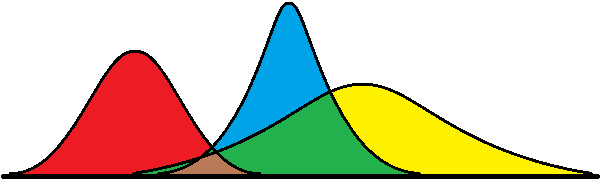
\includegraphics[width=.7\columnwidth]{GaussianDistOverlap1D.png}}
	}
\caption{A similarity index between three Gaussian distributions is illustrated as summation of overlapping regions of two distributions (green) or three distributions (brown).
This concept is easily extended to multivariate distributions.
}\label{fig:SimMeas}
\end{figure}

	
\subsection{Optimal Coalescence Avoidance}

Soft decision algorithms such as the JPDAF and MUJPDAF, which only consider estimate uncertainties when determining estimator gains, yield coalescence among the estimates.
However, including a similarity index in an optimal fashion to determine each gain matrix serves to remove this coalescence.
Let $\mathbf{J}\in\Re$ be a cost function of coalescence avoiding filtering as
\begin{align}
\mathbf{J}=J_P+cJ_S,
\end{align}
where $J_P$ is an uncertainty cost that measures the confidence level of the estimates and $J_S$ is a similarity cost that measures a degree of coalescence. The constant $c$ is a positive weighting factor between $J_P$ and $J_S$. 
The estimator gain $K_i$ is selected to minimize the total cost $\mathbf{J}$.
In short, the estimator gain is chosen in the consideration of both uncertainty and coalescence, illustrated in Figure \ref{fig:CostTrends}.


\begin{figure}
\setlength{\unitlength}{0.05\columnwidth}
\centerline{\footnotesize\selectfont
\begin{picture}(8.5,7.3)(-0.5,-0.8)
\put(-0.5,3){\rotatebox{90}{Cost}}
\put(0,0){\includegraphics[width=0.4\columnwidth]{ECC14_fig1.pdf}}
\put(5.3,1.2){\shortstack[c]{Uncertainty\\ cost: $J_P$}}
\put(6.2,2.6){\shortstack[c]{Similarity\\ cost: $J_S$}}
\put(5.2,5.2){\shortstack[c]{Weighted sum:\\ $\mathbf{J}=J_P+cJ_S$}}
\put(4.98,0.78){\circle*{0.1}}
\put(2.48,1.57){\circle*{0.1}}
\put(4.8,-0.4){$K_{MUJPDAF}$}
\put(2.3,-0.4){$K_{C-JPDAF}$}
\put(3.1,-0.8){Estimator gain}
\end{picture}
}
\caption{Illustration of optimal coalescence avoidance: several costs are illustrated with respect to an element of an estimator gain $K$ (red: uncertainty cost $J_P$, blue: similarity cost $J_S$, black: weighted sum). The estimator gain $K_{MUJPDAF}$ is selected to minimize the uncertainty cost. The estimator gain $K_{C-JPDAF}$ is chosen such that the weighted sum of the uncertainty cost and the similarity cost is minimized. In short, at the expense of increased uncertainty at a single step, the proposed approach prevents coalescence. The increased uncertainty at each step is rewarded by reducing the overall estimation error drastically by maintaining correct data association during close proximity tracking scenarios or missions.}
\label{fig:CostTrends}
\end{figure}

\paragraph*{Uncertainty Cost}
The uncertainty cost $J_P$ is defined as the sum of the trace of each posterior covariance:
\begin{align}
J_P=\sum\limits_{i}\tr{P^+_i},\label{eqn:JP}
\end{align}
where $P^+_{i}$ is obtained by \refeqn{JPDAFCov}.
Therefore, $P_i$ does not depend on $K_j$ for $i\neq j$.
The derivative of $J_P$ is taken from \refeqn{Uncertainty0}
\begin{align}
\label{eqn:CostP}
\frac{\partial J_{P}}{\partial K_{i}}&=2K_iE_i-2(1-\beta_{0,i})P^-_iH_i^T.
\end{align}

\paragraph*{Similarity Cost}
Any shared measurement $z_j$ on measurement estimate $\hat z_i$ yields an innovation $e_{ij}$ according to \refeqn{eij}.
During the measurement update, this innovation typically has the net effect of drawing $\hat z_i$ towards $z_j$ if $\beta_{ij}$ is nonzero.
This occurs for all estimates and all measurements; coalescence results when measurement estimates are drawn towards common measurements.
Therefore, coalescence of the JPDAF or MUJPDAF occurs inside the measurement space (e.g. if a sensor provides ranges and bearings, these are in the measurement space as opposed to a Cartesian state vector inside the state space).
Contrary to~\cite{KauLovLee14} where the similarity index is in terms of state space variables, the coalescence avoidance presented in this paper takes place inside the measurement space to most directly remove the coalescence.
Let the posterior measurement estimate be $\hat z_i^+\in\Re^m$ and its innovation be $e_{i}^+\in\Re^m$ that corresponds with its true measurement $z_i\in\Re^m$ (although association is unknown) as
\footnote{See the footnote on page~\pageref{fn:nonlinsys} for nonlinear systems.}
\begin{align}
\hat z_i^+&=H_i\hat x_i^+,
\\
e_{i}^+&=z_i-\hat z_i^+=(H_ix_i+v_i)-H_i\hat x_{i}^+=H_i\tilde x_i^++v_i,
\end{align}
where $\tilde x_i^+=x_i-\hat x_{i}^+$ denotes the error between the true state and the posterior estimate. The posterior innovation covariance $S^+_i\in\Re^{m\times m}$ is given by
\begin{align}
S^+_i&=\mathrm{E}[e_i^+e_i^{+T}]=\mathrm{E}[(H_i\tilde x_i^++v_i)(H_i\tilde x_i^++v_i)^T]\nonumber
\\
&=H_i\mathrm{E}[\tilde x_i^+\tilde x_i^{+T}]H_i^T+\mathrm{E}[vv^T]\nonumber%asdf
\\
&=H_iP^+_iH_i^T+R_i.
\end{align}
From these, the similarity cost is defined according to the format of \refeqn{zetaGeneral} as
%which are used to define $u_{p q}$ between $\hat z^+_{p}$ and $\hat z^+_{q}$:
\begin{align}
\label{eqn:Js}
J_S&=\sum\limits_{p,q\in I,p\neq q}\exp (-au_{pq}),
\end{align}
where $u_{pq}\in\Re$ is
\begin{align}
u_{pq} & = (\hat z_{p}^+-\hat z^+_{q})^T{S^+_{pq}}^{-1}(\hat z^+_{p}-\hat z^+_{q})\label{eqn:U},
\end{align}
where $S^+_{pq}=S^+_{p}+S^+_{q}$. Expanding \refeqn{U} with respect to the $p$-th system,
\begin{align}
u_{pq}=&\ 
(H_pK_p{\bf\bar e}_p-\hat z^+_{q})^T
(H_pP^+_{p}H_p^T+R_p+S^+_q)^{-1}  
(H_pK_p{\bf\bar e}_p-\hat z^+_{q}).
\end{align}

Next, we find the derivative of the similarity cost as follows.
Let $\Ibd\in \Re^{n\times m}$ be defined such that its $b,d$-th element is one and other elements are zero.
The partial derivative of $u_{pq}$ with respect to the scalar value at the $b,d$-th element of $K_p$, denoted as $K_{p,bd}$, is
\begin{align}
\deriv{u_{pq}}{K_{p,bd}}
=&\ 
(H_p\Ibd{\bf\bar e}_p)^T
{S_{pq}}^{-1}
(H_pK_p{\bf\bar e}_p-\hat z^+_{q})+
(H_pK_p{\bf\bar e}_p-\hat z^+_{q})^T
\mathcal{S}
(H_pK_p{\bf\bar e}_p-\hat z^+_{q})\nonumber
\\
&\ +
(H_pK_p{\bf\bar e}_p-\hat z^+_{q})^T
{S_{pq}}^{-1}
(H_p\Ibd{\bf\bar e}_p)\nonumber
\\
=&\ \{
2(H_p\Ibd{\bf\bar e}_p)^T
{S_{pq}}^{-1} +(H_pK_p{\bf\bar e}_p-\hat z^+_{q})^T
\mathcal{S}
\}(H_pK_p{\bf\bar e}_p-\hat z^+_{q}),\label{eqn:derivu}
\\
\deriv{u_{pq}}{K_{r,bd}}=&\ 0\quad \mbox{if } r\not\in\{p,q\},\label{eqn:derivu0}
\end{align}
where
\begin{align}
\mathcal{S}=&\ \deriv{{S^+_{pq}}^{-1}}{K_{p,bd}}\nonumber
\\
=&\ -{S^+_{pq}}^{-1}
\deriv{\left(H_pP^+_{p}H_p^T+R_p+S^+_q\right)}{K_{p,bd}}
{S^+_{pq}}^{-1}\nonumber
\\
=&\ -{S^+_{pq}}^{-1}
H_p
[(1-\beta_{0,p})(\Ibd H_pP_p^-+P_p^-H_p^T\Ibd^T)-\Ibd E_pK_p^T -K_pE_p\Ibd^T]
H_p^T
{S^+_{pq}}^{-1},\label{eqn:SS}
\end{align}
because
\begin{align}
&\deriv{\left(H_pP^+_{p}H_p^T+R_p+S^+_q\right)}{K_{p,bd}}
=
H_p
\deriv{P^+_{p}}{K_{p,bd}}
H_p^T\nonumber
\\
&=
H_p
[(1-\beta_{0,p})(\Ibd H_pP_p^-+P_p^-H_p^T\Ibd^T)-\Ibd E_pK_p^T -K_pE_p\Ibd^T]
H_p^T.\label{eqn:SSmidpart}
\end{align}
Then, \refeqn{SS} and \refeqn{SSmidpart} are substituted into \refeqn{derivu} or \refeqn{derivu0} to solve
\begin{align}
\label{eqn:JSK}
\deriv{J_S}{K_{p,bd}}=\ -a\sum\limits_{q\in I,q\neq p}\exp (-au_{pq})\deriv{u_{pq}}{K_{p,bd}}.
\end{align}

Necessary conditions for optimality are given by
\begin{align}
\deriv{\mathbf{J}}{K_i} = \deriv{J_P}{K_i} + c \deriv{J_S}{K_i} =0,\label{eqn:NCO}
\end{align}
where $\deriv{J_P}{K_i}$ and $\deriv{J_S}{K_i}$ may be nonzero.
In short, \refeqn{CostP} and \refeqn{JSK} are substituted into \refeqn{NCO} and repeated for all $p$ to obtain the set of optimal gains $\mathcal{K}=\{K_1,K_2,...,K_{n_t}\}$.
Then, the C-JPDAF is completed by updating the state estimate and covariance by using \refeqn{KalEst} and \refeqn{JPDAFCov}, respectively.
As the optimality condition is a nonlinear function of estimator gains, there is no closed-form solution.
Hence, we require a nonlinear equation solver.
When $c=0$, we can show that the optimal gain reduces to that of the MUJPDAF, which is used as an initial guess of numerical solutions.
Therefore, if the number of estimates exhibiting significant similarity is $n_t^*\leq n_t$ and $\mathcal C$ is the number of times \refeqn{NCO} is solved depending on the numerical accuracy, then the required iterations is $n_t^*(n_t^*-1)\mathcal C$, where some variables may be reused (e.g. $S^+_{pq}\equiv S^+_{qp}$) and often the effect of \refeqn{derivu} is negligible.





\section{Numerical Examples}

We consider satellites in the lower earth orbit (LEO) and in the geosynchronous orbit (GEO) to compare the performances of the conventional JPDAF, the MUJPDAF, and the C-JPDAF, using equations of motion based off the two-body problem.

Let $\vec r=\begin{bmatrix}x_1 & x_2 & x_3\end{bmatrix}^T$ be the position vector of the $i$-th satellite represented with respect to the Earth-Centered Inertial (ECI) frame.
The equation of motion corresponding to the two-body problem is given by
\begin{align}
\ddot{\vec r}&=-\frac{\mu}{r^3}\vec r=-\mu(\vec r^T\vec r)^{-\frac32}\vec r,
\end{align}
where $\mu=398,600\ \frac{km^3}{sec^2}$ is the gravitational constant of the earth if position is estimated in kilometers and time is measured in seconds~\cite{Val01}.

Let $\delta$ denote an infinitesimal change of a state variable.
The linearized equations of state variable $\vec x=\begin{bmatrix}\vec r^T, & \dot{\vec r}^T\end{bmatrix}^T\in\Re^6$ are given by
\begin{align}
\begin{bmatrix}
\delta\dot{\vec r} \\ \delta\ddot{\vec r}
\end{bmatrix}
%\delta\dot{\vec x}
=
\begin{bmatrix}
0_{3\times3} & I_{3\times3} \\
\mu\left[3\vec r({\vec r}^T\vec r)^{-\frac52}{\vec r}^T-({\vec r}^T\vec r)^{-\frac32}I_{3\times3}\right] & 0_{3\times3}
\end{bmatrix}
\begin{bmatrix}
\delta\vec r \\ \delta\dot{\vec r}
\end{bmatrix}
%\delta\vec x
.
\end{align}
%Defining the above square matrix as $A_{lin}$, the linearized state transition matrix over the time step $dt$ is defined as
%\begin{align}
%F=\expm{(A_{lin}dt)}
%\end{align}
%where $\expm$ denotes the matrix exponential function.

The process uncertainty may be subject to a variety of perturbations beyond two-body forces, and the process covariance takes the form $Q=\diag[\sigma_r^2I_{3\times3}, \sigma_{\dot r}^2I_{3\times3}]$, which varies depending on the case considered.
%=\diag[10^{-6}I_{3\times3}, 10^{-8}I_{3\times3}]$.

For the cases where the satellites are orbiting in LEO, the satellites are measured with a single phased-array radar at location $x_s$ on the equator
\begin{align}
x_s=
\begin{bmatrix}
R_E\cos\frac{2\pi t}T & R_E\sin\frac{2\pi t}T & 0 & -\frac{2\pi tR_E}T\sin\frac{2\pi t}T  & \frac{2\pi tR_E}T\cos\frac{2\pi t}T & 0
\end{bmatrix}^T,
\end{align}
where $R_E=6378$ km is the radius of the earth, time of the day $t$ starts at $0$ seconds, and the time period of a day of the day is $T=86164.090518$ seconds.
Here, the measurement space consists of the range $\rho$ between the sensor and the satellite (km), the range rate $\dot\rho$ (km/sec), and topocentric right ascension $\alpha$ and declination $\delta$ (rad)~\cite{Val01}.
The standard deviations $\sigma_\rho$, $\sigma_\alpha$, and $\sigma_\delta$ are based on the Mahe Ground Station uncertainty data~\cite{VerSauSco04} and $\sigma_{\dot\rho}$ from paper examples~\cite{KurAriAriEfe10}.
The measurement uncertainty is $R=\diag[\sigma_\rho^2, \sigma_{\dot\rho}^2, \sigma_\alpha^2, \sigma_\delta^2]=\diag[0.15^2, 0.005^2, (\frac{0.01\pi}{180})^2, (\frac{0.01\pi}{180})^2]$.
For GEO, angles-only measurements are available with higher accuracy; namely the topocentric right ascension and declination are chosen as $\sigma_{\alpha,GEO}=\sigma_{\delta,GEO}=10^{-2}\sigma_\alpha$.
For all cases, there is a $10\%$ chance that a measurement is either deleted or an extraneous measurement is added at each time step.
These cases are outlined in Table \ref{tab:CaseDef}.

Further descriptions of the cases are available below, and the resulting accuracy is measured with RMS error, the uncertainty is summarized with $\tr{J_P}$, and the computation time is measured as well, tabulated in Tables \ref{tab:A1}--\ref{tab:B2}.

\begin{table}
\begin{center}
\caption{Case Definitions} \label{tab:CaseDef}
\begin{threeparttable}[h]
\begin{tabularx}{.59\textwidth}
{
>{$}c<{$} |
>{$}c<{$}
}
\toprule
\multirow{2}{*}{Symbol} & \multirow{2}{*}{Explanation}\\
\\
\midrule
\multirow{1}{*}{A} &  \multirow{1}{*}{Comparison of JPDAF and MUJPDAF}
\\
\multirow{1}{*}{B} &  \multirow{1}{*}{Comparison of JPDAF, MUJPDAF, and C-JPDAF}
\\
\multirow{1}{*}{1} &  \multirow{1}{*}{Orbits in LEO}
\\
\multirow{1}{*}{2} &  \multirow{1}{*}{Orbits in GEO}
\\
\multirow{1}{*}{a} &  \multirow{1}{*}{$\sigma^2_{r,a} = \epsilon\sigma^2_{r}$}
\\
\multirow{1}{*}{b} &  \multirow{1}{*}{$\sigma^2_{\dot r,b} = \epsilon\sigma^2_{\dot r}$}
\\
\multirow{1}{*}{c} &  \multirow{1}{*}{$\sigma^2_{r,c} = \epsilon\sigma^2_{r}$, $\sigma^2_{\dot r,c} = \epsilon\sigma^2_{\dot r}$}
\\
\multirow{1}{*}{d} &  \multirow{1}{*}{$\sigma^2_{\alpha,d} = \epsilon\sigma^2_{\alpha}$, $\sigma^2_{\delta,d} = \epsilon\sigma^2_{\delta}$}
\\
\multirow{1}{*}{e} &  \multirow{1}{*}{$\sigma^2_{\mathbf{range},e} = \epsilon\sigma^2_{\mathbf{range}}$ (case number 1 only)}
\\
\multirow{1}{*}{f} &  \multirow{1}{*}{$\sigma^2_{\mathbf{range-rate},f} = \epsilon\sigma^2_{\mathbf{range-rate}}$ (case number 1 only)}
\\
\bottomrule
\end{tabularx}
\end{threeparttable}
\end{center}
\end{table}


% Alan's note:
%The scenarios below (A and B) are those from the ACC paper submission; the results to be included in this paper are according to those outlined in Table 1.
%The brief summary of these results to come is that the minimum uncertainty JPDAF (MUJPDAF) outperforms the conventional JPDAF in every case (LEO and GEO) in terms of reducing uncertainty and improving state estimate accuracy, and the coalescence-avoiding optimal JPDAF (C-JPDAF) often outperforms the MUJPDAF and JPDAF in both LEO and GEO scenarios in terms of state estimate accuracy only, but this is not always guaranteed.




\paragraph*{Scenario A1: Comparison of the JPDAF and MUJPDAF with two LEO satellites in close proximity}

The first set of cases compares the JPDAF with the MUJPDAF for tracking two nearby satellites passing over the sensor field of view in LEO. The initial conditions of the first two orbits are chosen as
\begin{align}
x_{1,A1}=x_{ref,A1}+x_{pert,A1},& \quad x_{2,A1}=x_{ref,A1}-x_{pert,A1},\nonumber
\\
x_{ref,A1}=\begin{bmatrix}7000 & 0 & 1000 & 0 & 7.546 & 0\end{bmatrix}^T,& \quad x_{pert,A1}=\begin{bmatrix}
0.2 & 0 & 0 & 0 & -0.105 & 0
\end{bmatrix}^T.
\end{align}
In these cases, the process covariance is $Q=\diag[10^{-6}I_{3\times3}, 10^{-8}I_{3\times3}]$, the estimates have initial covariances matrix $P_{0,A1}=10^7\times Q$, time steps of $1$ second over $100$ seconds, and $\epsilon=10$.
These scenarios are chosen because the estimates exhibit large initial uncertainties, so the spread in the innovations affects the updates.
The gain of the MUJPDAF accounts for this portion of the state covariance matrix better than the gain for the conventional JPDAF in every single case.
Given identical parameters and measurements, the RMS errors of the position are lower in \emph{every} case when the MUJPDAF is applied compared with when the conventional JPDAF is applied.
In fact in two cases, namely A1b and A1c, the JPDAF is incapable of decreasing the estimate uncertainty as quickly as the MUJPDAF; the JPDAF initially suffers from such great coalescence that the estimates become associated with incorrect measurements consistently.
Furthermore, the computational time is roughly the same between the JPDAF and MUJPDAF, so the results suggest that the improvement in accuracy is at no increase in computation.
These results are tabulated in Table \ref{tab:A1}, and some cases are plotted in Figure \ref{fig:A1}.


\begin{center}
\begin{threeparttable}[h]
\caption{Cases of A1} \label{tab:A1}
\begin{tabularx}{.58\textwidth}
{
>{$}c<{$} |
*{2}{>{$}c<{$}} |
*{2}{>{$}c<{$}}
}
\toprule
\multirow{2}{*}{Case} & \multicolumn{2}{c}{\multirow{1}{*}{RMS Position Error (km)}} & \multicolumn{2}{c}{\multirow{1}{*}{Time (sec)}} \\
 & \multirow{1}{*}{JPDAF} & \multirow{1}{*}{MUJPDAF} & \multirow{1}{*}{JPDAF} & \multirow{1}{*}{MUJPDAF}
\\
\midrule
A1  & 0.12026 & 0.10646 & 0.582294 & 0.560754 \\
A1a & 0.17910 & 0.17157 & 0.558011 & 0.561458 \\
A1b & \hilight{2.63710} & 0.14150 & 0.561605 & 0.558537 \\
A1c & \hilight{2.63520} & 0.19559 & 0.570204 & 0.578704 \\
A1d & 0.20204 & 0.18865 & 0.572659 & 0.578029 \\
A1e & 0.14541 & 0.13361 & 0.575572 & 0.573995 \\
A1f & 0.12175 & 0.10795 & 0.576113 & 0.559978 \\
\bottomrule
\end{tabularx}
{\small
\begin{tablenotes}
    \item \hilight{Track swapping occurs}
  \end{tablenotes}}
\end{threeparttable}
\end{center}


\begin{figure}
{
%\hspace*{0.05\columnwidth}
\centerline{
	\subfigure[\;Case A1: JPDAF]
		{\hspace*{0.\columnwidth}\includegraphics[width=0.5\columnwidth]{A1JPDAF.pdf}}
	\subfigure[\;Case A1: MUJPDAF]
		{\hspace*{0.\columnwidth}\includegraphics[width=0.5\columnwidth]{A1MUJPDAF.pdf}}
	}
\centerline{
	\subfigure[\;Case A1b: JPDAF]
		{\hspace*{0.\columnwidth}\includegraphics[width=0.5\columnwidth]{A1bJPDAF.pdf}}
	\subfigure[\;Case A1b: MUJPDAF]
		{\hspace*{0.\columnwidth}\includegraphics[width=0.5\columnwidth]{A1bMUJPDAF.pdf}}
	}
\centerline{
	\subfigure[\;Case A1d: JPDAF]
		{\hspace*{0.\columnwidth}\includegraphics[width=0.5\columnwidth]{A1dJPDAF.pdf}}
	\subfigure[\;Case A1d: MUJPDAF]
		{\hspace*{0.\columnwidth}\includegraphics[width=0.5\columnwidth]{A1dMUJPDAF.pdf}}
	}
}
\caption{The orbital radii of three cases are shown where the dashed plots are the true trajectories and the solid plots are the estimated trajectories.
In all cases the MUJPDAF is more accurate and experiences less coalescence than the JPDAF.
In particular, when the JPDAF is used in to Case A1b, the initial coalescence causes track swapping.
Additionally, Case A1d experiences the most inaccurate estimation without track swapping with very noisy angle measurements.
}\label{fig:A1}
\end{figure}















\paragraph*{Scenario A2: Comparison of the JPDAF and MUJPDAF with two near-GEO satellites in close proximity}

The second set of cases compares the JPDAF with the MUJPDAF for tracking two nearby satellites passing over the sensor field of view in GEO, where the orbital radius is $r_{GEO}=4.2164\times10^{4}\ km$. The initial conditions of the first two orbits are chosen as
\begin{align}
x_{1,A2}&=\begin{bmatrix}r_{GEO} & 0 & 0 & 0 & \sqrt{\frac{\mu}{r_{GEO}}}, & 0\end{bmatrix}^T,
\\
x_{2,A2}&=x_{1,A2}+\begin{bmatrix}
0 & 0 & -1 & 0 & 0 & 4\times10^{-4}
\end{bmatrix}^T,
\end{align}
or where $x_{1,A2}$ remains exactly in GEO while $x_{2,A2}$ starts slightly perturbed from a GEO orbit with a nonzero inclination such that the two satellites nearly collide as they pass by in close proximity.
Unlike the last cases, the A2 cases consider small initial covariance matrices $P_{0,A2}= Q$ where $Q=\diag[10^{-6}I_{3\times3}, 10^{-8}I_{3\times3}]$, time steps of $10$ seconds over $5000$ seconds, and $\epsilon=1.1$.
%These scenarios are chosen because the estimates exhibit large initial uncertainties, so the spread in the innovations affects the updates.
Even though the initial conditions are largely different from those of the A1 cases, the A2 cases display the same trends, where the computational costs among the algorithms are roughly the same but the tracking abilities of the MUJPDAF \emph{always} yield estimates closer to the truth than those of the JPDAF.
These results are tabulated in Table \ref{tab:A2}, and some cases are plotted in Figure \ref{fig:A2}.

\begin{center}
\begin{threeparttable}[h]
\caption{Case A2} \label{tab:A2}
\begin{tabularx}{.65\textwidth}
{
>{$}c<{$} |
*{2}{>{$}c<{$}} |
*{2}{>{$}c<{$}}
}
\toprule
\multirow{2}{*}{Case} & \multicolumn{2}{c}{\multirow{1}{*}{RMS Angular Error (rad)}} & \multicolumn{2}{c}{\multirow{1}{*}{Time (sec)}} \\
 & \multirow{1}{*}{JPDAF} & \multirow{1}{*}{MUJPDAF} & \multirow{1}{*}{JPDAF} & \multirow{1}{*}{MUJPDAF}
\\
\midrule
A2  & 1.2140\times10^{-6} & 9.8784\times10^{-7} & 2.765200 & 2.732202 \\
A2a & 1.2141\times10^{-6} & 9.8780\times10^{-7} & 2.739866 & 2.743265 \\
A2b & \hilight{1.1728$\times10^{-5}$} & 1.0143\times10^{-6} & 2.733589 & 2.742162 \\
A2c & \hilight{1.1728$\times10^{-5}$} & 1.0142\times10^{-6} & 2.732890 & 2.751087 \\
A2d & \hilight{1.1700$\times10^{-5}$} & 1.0332\times10^{-6} & 2.819630 & 2.773270 \\
\bottomrule
\end{tabularx}
{\small
\begin{tablenotes}
    \item \hilight{Track swapping occurs}
  \end{tablenotes}}
\end{threeparttable}
\end{center}

\begin{figure}
{
%\hspace*{0.05\columnwidth}
\centerline{
	\subfigure[\;Case A2: JPDAF]
		{\hspace*{0.\columnwidth}\includegraphics[width=0.5\columnwidth]{A2JPDAF.pdf}}
	\subfigure[\;Case A2: MUJPDAF]
		{\hspace*{0.\columnwidth}\includegraphics[width=0.5\columnwidth]{A2MUJPDAF.pdf}}
	}
\centerline{
	\subfigure[\;Case A2a: JPDAF]
		{\hspace*{0.\columnwidth}\includegraphics[width=0.5\columnwidth]{A2aJPDAF.pdf}}
	\subfigure[\;Case A2a: MUJPDAF]
		{\hspace*{0.\columnwidth}\includegraphics[width=0.5\columnwidth]{A2aMUJPDAF.pdf}}
	}
\centerline{
	\subfigure[\;Case A2b: JPDAF]
		{\hspace*{0.\columnwidth}\includegraphics[width=0.5\columnwidth]{A2bJPDAF.pdf}}
	\subfigure[\;Case A2b: MUJPDAF]
		{\hspace*{0.\columnwidth}\includegraphics[width=0.5\columnwidth]{A2bMUJPDAF.pdf}}
	}
}
\caption{The orbital radii of three cases are shown where the dashed plots are the true trajectories and the solid plots are the estimated trajectories and $\alpha_{diff}$ is the difference between $\alpha_{1}$ and $\hat\alpha_{1,A2}$ or $\hat\alpha_{2,A2}$.
Cases A2 and A2a serve as examples where the coalescence during crossing periods with the JPDAF yields much more similar estimates than with the MUJPDAF.
In Case A2b, this coalescence is so severe that track swapping occurs with the JPDAF, but this is avoided with the MUJPDAF.
}\label{fig:A2}
\end{figure}




















\paragraph*{Scenario B1: Comparison of the JPDAF, MUJPDAF, and C-JPDAF with three LEO satellites in close proximity}
The JPDAF, MUJPDAF, and C-JPDAF algorithms are compared for three satellites in LEO with initial conditions
\begin{align}
\begin{split}
x_{1,B1}&=x_{ref,B1}+x_{pert,B1}, \quad x_{2,B1}=x_{ref,B1}-x_{pert,B1}, \quad x_{3,B1}=x_{ref,B1},
\\
x_{ref,B1}&=\begin{bmatrix}7000 & 0 & 0 & 0 & 7.546 & 0\end{bmatrix}^T, \quad x_{pert,B1}=\begin{bmatrix}
0.025 & 0 & 0 & 0 & 0 & 0
\end{bmatrix}^T,
\end{split}
\end{align}
where $Q=\diag[10^{-6}I_{3\times3}, 10^{-8}I_{3\times3}]$, $P_{0,B1}=Q$, and $\epsilon=1.1$ for time steps of $10.0$ seconds over a $2000$ second time period.
This corresponds to a phased-array radar observing observing a slow separation of objects in a near-circular orbit; because the satellite states are in close proximity over a large time period, the JPDAF and MUJPDAF are subject to severe coalescence.
The C-JPDAF is designed to avoid this coalescence, where the parameters $a=5\times10^{-1}$ and $c=2.3\times10^{-4}$ are used in these scenarios.
The accuracy of the C-JPDAF is largely improved from that of the JPDAF and MUJPDAF; however, the computational cost of the C-JPDAF is roughly $60$ times that of either other algorithm.
The position RMS error and computation time are tabulated in Table \ref{tab:B1} and some example plots from these cases are shown in Figure \ref{fig:B1}.

\begin{center}
\begin{threeparttable}[h]
\caption{Case B1} \label{tab:B1}
\begin{tabularx}{.81\textwidth}
{
>{$}c<{$} |
*{3}{>{$}c<{$}} |
*{3}{>{$}c<{$}}
}
\toprule
\multirow{2}{*}{Case} & \multicolumn{3}{c}{\multirow{1}{*}{RMS Position Error (km)}} & \multicolumn{3}{c}{\multirow{1}{*}{Time (sec)}} \\
 & \multirow{1}{*}{JPDAF} & \multirow{1}{*}{MUJPDAF} & \multirow{1}{*}{C-JPDAF} & \multirow{1}{*}{JPDAF} & \multirow{1}{*}{MUJPDAF} & \multirow{1}{*}{C-JPDAF}
\\
\midrule
B1   	& 0.14432 & 0.091133 & 0.057312 & 1.736272 & 1.670539 & 101.000529 \\
B1a 	& 0.14432 & 0.091134 & 0.057307 & 1.689807 & 1.726980 & 100.988662 \\
B1b 	& 0.14694 & 0.094506 & 0.055145 & 1.673762 & 1.678786 & 100.855376 \\
B1c 	& 0.14693 & 0.094507 & 0.055136 & 1.675486 & 1.669083 & 100.907850 \\
B1d 	& 0.14400 & 0.088933 & 0.058911 & 1.663424 & 1.660136 & 102.606102 \\
B1e 	& 0.14408 & 0.090823 & 0.059919 & 1.673660 & 1.666829 & 100.278073 \\
B1f 	& 0.14436 & 0.091212 & 0.064299 & 1.732541 & 1.721413 & 98.672870 \\
\bottomrule
\end{tabularx}
\end{threeparttable}
\end{center}

\begin{figure}
{
%\hspace*{0.05\columnwidth}
\centerline{
	\subfigure[\;Case B1: JPDAF]
		{\hspace*{0.\columnwidth}\includegraphics[width=0.33\columnwidth]{B1JPDAF.pdf}}
	\subfigure[\;Case B1: MUJPDAF]
		{\hspace*{0.\columnwidth}\includegraphics[width=0.33\columnwidth]{B1MUJPDAF.pdf}}
	\subfigure[\;Case B1: C-JPDAF]
		{\hspace*{0.\columnwidth}\includegraphics[width=0.33\columnwidth]{B1C-JPDAF.pdf}}
	}
\centerline{
	\subfigure[\;Case B1c: JPDAF]
		{\hspace*{0.\columnwidth}\includegraphics[width=0.33\columnwidth]{B1cJPDAF.pdf}}
	\subfigure[\;Case B1c: MUJPDAF]
		{\hspace*{0.\columnwidth}\includegraphics[width=0.33\columnwidth]{B1cMUJPDAF.pdf}}
	\subfigure[\;Case B1c: C-JPDAF]
		{\hspace*{0.\columnwidth}\includegraphics[width=0.33\columnwidth]{B1cC-JPDAF.pdf}}
	}
\centerline{
	\subfigure[\;Case B1f: JPDAF]
		{\hspace*{0.\columnwidth}\includegraphics[width=0.33\columnwidth]{B1fJPDAF.pdf}}
	\subfigure[\;Case B1f: MUJPDAF]
		{\hspace*{0.\columnwidth}\includegraphics[width=0.33\columnwidth]{B1fMUJPDAF.pdf}}
	\subfigure[\;Case B1f: C-JPDAF]
		{\hspace*{0.\columnwidth}\includegraphics[width=0.33\columnwidth]{B1fC-JPDAF.pdf}}
	}
}
\caption{The orbital radii of three cases are shown where the dashed plots are the true trajectories and the solid plots are the estimated trajectories.
In all cases the MUJPDAF is more accurate and experiences less coalescence than the JPDAF, but both algorithms suffer from coalescence.
The C-JPDAF systematically removes this coalescence from the updates at the cost of slightly larger covariance matrices and a large increase in required computational resources.
%Between Cases B1 and B1c, the process position uncertainty is increased, which last little effect on the estimates since this has little
The conditions that affect the C-JPDAF most are with Case B1f where the range-rate measurements have the greatest uncertainty.
}\label{fig:B1}
\end{figure}

Among the variations of the B1 cases, the range-rate measurement uncertainty (Case B1f) has the largest effect on tracking with the C-JPDAF.
In the B1 cases, the ranges and bearings of each track are close and changing, but the difference between the velocities of the three satellites remain largely constant after about $500$ seconds.
As long as the estimates are able to stay sufficiently far apart, as the C-JPDAF is able to accomplish, the component of the velocity measurement in the radial direction serves as a distinguishing portion of the full measurement, so that the correct association between measurement and estimate is more heavily weighted, and hence better tracking is achieved.
The quality of the range-rate measurement is degraded in Case B1f, and hence the C-JPDAF algorithm is not able to as accurately track each estimate when compared with the other B1 cases.



















\paragraph*{Scenario B2: Comparison of the JPDAF, MUJPDAF, and C-JPDAF with two GEO satellites in close proximity}
The JPDAF, MUJPDAF, and C-JPDAF algorithms are compared for two satellites in GEO with initial conditions
\begin{align}
\begin{split}
x_{1,B2}&=f_{GEO}(0^\circ), \quad x_{2,B2}=f_{GEO}({10^{-4}}^\circ), \quad \mbox{where}
\\
f_{GEO}(\theta)&=\begin{bmatrix}r_{GEO}\cos\theta & r_{GEO}\sin\theta & 0 & \sqrt{\frac{\mu}{r_{GEO}}}\cos(90^\circ+\theta) & \sqrt{\frac{\mu}{r_{GEO}}}\sin(90^\circ+\theta) & 0\end{bmatrix}^T,
\end{split}
\end{align}
where $Q=\diag[10^{-8}I_{3\times3}, 10^{-10}I_{3\times3}]$, $P_{0,B}=Q$, and $\epsilon=1.1$ for time steps of $10.0$ seconds over a $2000$ second time period.
This corresponds to a scenario where two satellite orbit steadily nearby in GEO.
For the C-JPDAF, the parameters $a=1.5\times10^{2}$ and $c=1\times10^{10}$ are used in these scenarios.
In theory, topocentric right ascension measurements should be the same distance apart throughout the cases and the declination should always be zero.
Much like the B1 cases, the accuracy of the C-JPDAF yields a large improvement from that of the JPDAF and MUJPDAF; however, the increase in computational cost of the C-JPDAF is roughly $30$ times that of either other algorithm, which is about half of the increase found with the B1 cases.
This is because the similarity measure of two estimates is less complex with the B2 cases than with three estimates in the B1 cases.
The angular RMS error and computation time are tabulated in Table \ref{tab:B2} and some example plots from these cases are shown in Figure \ref{fig:B2}.




\begin{center}
\begin{threeparttable}[h]
\caption{Case B2} \label{tab:B2}
\begin{tabularx}{.95\textwidth}
{
>{$}c<{$} |
*{3}{>{$}c<{$}} |
*{3}{>{$}c<{$}}
}
\toprule
\multirow{2}{*}{Case} & \multicolumn{3}{c}{\multirow{1}{*}{RMS Angular Error (rad)}} & \multicolumn{3}{c}{\multirow{1}{*}{Time (sec)}} \\
 & \multirow{1}{*}{JPDAF} & \multirow{1}{*}{MUJPDAF} & \multirow{1}{*}{C-JPDAF} & \multirow{1}{*}{JPDAF} & \multirow{1}{*}{MUJPDAF} & \multirow{1}{*}{C-JPDAF}
\\
\midrule
B2   	& 1.1112\times10^{-6} & 9.4780\times10^{-7} & 5.6708\times10^{-7} & 1.149378 & 1.119439 & 34.318254 \\
B2a 	& 1.1112\times10^{-6} & 9.4779\times10^{-7} & 5.6347\times10^{-7} & 1.154256 & 1.150072 & 34.758609 \\
B2b 	& 1.1306\times10^{-6} & 9.8287\times10^{-7} & 5.7387\times10^{-7} & 1.126598 & 1.132463 & 35.327683 \\
B2c 	& 1.1306\times10^{-6} & 9.8286\times10^{-7} & 5.6435\times10^{-7} & 1.118436 & 1.131690 & 34.817179 \\
B2d 	& 1.1115\times10^{-6} & 9.5439\times10^{-7} & 5.6136\times10^{-7} & 1.113892 & 1.116399 & 35.213445 \\
\bottomrule
\end{tabularx}
\end{threeparttable}
\end{center}

\begin{figure}
{
%\hspace*{0.05\columnwidth}
\centerline{
	\subfigure[\;Case B2: JPDAF]
		{\hspace*{0.\columnwidth}\includegraphics[width=0.33\columnwidth]{B2JPDAF.pdf}}
	\subfigure[\;Case B2: MUJPDAF]
		{\hspace*{0.\columnwidth}\includegraphics[width=0.33\columnwidth]{B2MUJPDAF.pdf}}
	\subfigure[\;Case B2: C-JPDAF]
		{\hspace*{0.\columnwidth}\includegraphics[width=0.33\columnwidth]{B2C-JPDAF.pdf}}
	}
\centerline{
	\subfigure[\;Case B2b: JPDAF]
		{\hspace*{0.\columnwidth}\includegraphics[width=0.33\columnwidth]{B2bJPDAF.pdf}}
	\subfigure[\;Case B2b: MUJPDAF]
		{\hspace*{0.\columnwidth}\includegraphics[width=0.33\columnwidth]{B2bMUJPDAF.pdf}}
	\subfigure[\;Case B2b: C-JPDAF]
		{\hspace*{0.\columnwidth}\includegraphics[width=0.33\columnwidth]{B2bC-JPDAF.pdf}}
	}
\centerline{
	\subfigure[\;Case B2d: JPDAF]
		{\hspace*{0.\columnwidth}\includegraphics[width=0.33\columnwidth]{B2dJPDAF.pdf}}
	\subfigure[\;Case B2d: MUJPDAF]
		{\hspace*{0.\columnwidth}\includegraphics[width=0.33\columnwidth]{B2dMUJPDAF.pdf}}
	\subfigure[\;Case B2d: C-JPDAF]
		{\hspace*{0.\columnwidth}\includegraphics[width=0.33\columnwidth]{B2dC-JPDAF.pdf}}
	}
}
\caption{In the various cases, the C-JPDAF is always able to produce more distinguishable estimates.
The perturbations among the cases yield slightly different results, but none are drastically different.
}\label{fig:B2}
\end{figure}

The most important result is that the C-JPDAF consistently avoids track-swapping, whereas the JPDAF and MUJPDAF do not.
However unlike the B1 cases, the B2 cases do not have a measurement that is consistently different among the estimates except for topocentric right ascension.
However, this component of the measurement is consistently very small.
Therefore, the variations from Case B2 all yield very close results.

An interesting observation from the data is the nonzero estimated declination, which should be zero because the GEO orbit lies on the equatorial plane; any shift from zero is due to process and measurement uncertainties.
Rather than observing independent errors among the two estimates, the declination errors are correlated and coalescing together.
The correlation of the sets of measurement estimates is easily explained by the soft decisions applied by all of the compared algorithms; measurement updates are largely shared among the estimates, so uncertainties affect the two estimates in a similar way.
Coalescence occurs when measurement updates are shared, shown in all cases in this paper, but the declination errors are less similar with the C-JPDAF.





\section{Conclusion}

The conventional JPDAF is a well-known algorithm with various applications in data association.
The soft decision approach makes the algorithm robust to missed detections and other clutter.
This paper enhances the JPDAF in two different ways.
First, the conventional JPDAF employs a Kalman gain, which does not minimize the trace of the state covariance matrix because the JPDAF yields an important spread in innovations term.
A minimum uncertainty JPDAF (MUJPDAF) is derived with a new gain that minimizes the full posterior uncertainty, including the spread in innovations state covariance matrix term.
This gain is computationally comparable to the JPDAF, and shows superior performance in estimate accuracy when the spread in the innovations is nonzero.

Second, both the JPDAF and the MUJPDAF involve measurement sharing, which tends to coalesce estimates in close proximity.
From~\cite{KauLovLee14}, the C-JPDAF is generalized for any number of estimates and measurements and the similarity cost is found inside the measurement space where coalescence occurs.
When using the C-JPDAF, there must be a trade-off between uncertainty increase and coalescence removal and powerful computational resources are also required.

The results in this paper show how the JPDAF, MUJPDAF, and C-JPDAF perform in LEO and GEO scenarios with various changes in parameters.
Numerous simulations show that the MUJPDAF operates at a similar computational cost to the JPDAF with a consistent improvement in accuracy.
In some scenarios where coalescence of the estimates is expected to be severe, the C-JPDAF can better track objects at the cost of increased computation.

Future work includes determining a systematic method of choosing the parameters for the C-JPDAF and deriving a suboptimal solution for the C-JPDAF that does not involve the large computation of the optimal solution.



\begin{appendix}
\label{append}

\subsection{Appendix A: Invertibility of the new $E_i$} \label{NewPartOfEIsPSD}
Consider that object $i$ is not measured (probability $\beta_{0,i}$), then this portion of the innovation update $e_0=0_{m\times1}$ because no innovation exists where measurements are not available.
Then for all innovations in the set $J^*=\{0\}\cup J$, the Total Probability Theorem holds true for object $i$:
\begin{align}
\sum\limits_{j^*\in J^*}\beta_{ij^*}=1.
\end{align}
From~\cite[Eq. 1.4.16-(1-10)]{ShaRonThi2001}, the covariance spread in the means term of the mixture of $e$ is defined as% (note that ${\bf e}_{i}$ remains unchanged)
\begin{align}
\tilde P_e=\sum\limits_{j^*}\beta_{ij^*}(e_{ij^*}-{\bf\bar e}_{i})(e_{ij^*}-{\bf\bar e}_{i})^T,
\end{align}
which is positive semi-definite. Manipulating this equation,
\begin{align}
\tilde P_e=&\sum\limits_{j^*}\beta_{ij^*}e_{ij^*}e_{ij^*}^T
-\sum\limits_{j^*}\beta_{ij^*}e_{ij^*}{\bf\bar e}_{i}^T
-{\bf\bar e}_{i}\sum\limits_{j^*}\beta_{ij^*}e_{ij^*}^T
+{\bf\bar e}_{i}{\bf\bar e}_{i}^T\nonumber%asdf
\\
=&\sum\limits_{j^*}\beta_{ij^*}e_{ij^*}e_{ij^*}^T-{\bf\bar e}_{i}{\bf\bar e}_{i}^T\nonumber
\\
=&\sum\limits_{j}\beta_{ij}e_{ij}e_{ij}^T-{\bf\bar e}_{i}{\bf\bar e}_{i}^T\geq0,
\label{eqn:CovSpreadPSD}
\end{align}
because $e_{i0}\equiv0$. Therefore $E_i$ is invertible $\forall\ 0\leq\beta_{0,i}<1$.


\subsection{Appendix B: The singularity of $E$ is not an infinite limit}
Consider the singularity when $E_i=0$ when no association is made to a track, or equivalently when $\beta^*=(1-\beta_{0,i})=\sum\limits_{j}\beta_j=0$.
It is clear from \refeqn{KalEst} and \refeqn{CovExpanded} that the updates are independent of $K_i$ exactly at this singularity.
We show that $K_i$ is \emph{not} growing without bound nearby this singularity, shown by evaluating the limit at this singularity to ensure boundedness.
Note that if $\sum\limits_{j}\beta_j\rightarrow0\Rightarrow \beta_j\rightarrow0\ \forall\ j$ because of the bounds $\sum\limits_{j}\beta_j\geq\beta_j\geq0\ \forall \ j$.
For clarity, let $\tilde\beta_p=\sum\limits_{j,j\neq p}\beta_j/\sum\limits_{j}\beta_j$ and drop the subscript $i$ because this analysis focuses on a single track.

First, we factor $\beta^*$ from $\sum\limits_{j} \beta_{j}e_{j}e_{j}^T$,
\begin{align}
\sum\limits_{j} \beta_{j}e_{j}e_{j}^T&=(\beta_1e_1e_1^T+\beta_2e_2e_2^T+\cdots)\nonumber
%\\
%&=\beta^*
%(e_1e_1^T-\tilde\beta_1e_1e_1^T+
%e_2e_2^T-\tilde\beta_2e_2e_2^T+\cdots),\nonumber
\\
&=\beta^*(\sum\limits_{j}e_{j}e_{j}^T-\sum\limits_{j}\tilde\beta_je_{j}e_{j}^T).
\end{align}
Similarly, we factor $\beta^*$ from ${{\bf\bar{e}}}{\bf\bar{e}}^T$,
\begin{align}
{{\bf\bar{e}}}{\bf\bar{e}}^T&=\sum\limits_{j} \beta_{j}e_{j}\sum\limits_{j} \beta_{j}e_{j}^T\nonumber%asdf
\\
%&=
%(\beta_1e_1\sum\limits_{j} \beta_{j}e_{j}^T+\beta_2e_2\sum\limits_{j} \beta_{j}e_{j}^T+\cdots),\nonumber
%\\
%&=\beta^*(e_1\sum\limits_{j} \beta_{j}e_{j}^T-\tilde\beta_1e_1\sum\limits_{j} \beta_{j}e_{j}^T\nonumber
%\\
%&\ \ \ +e_2\sum\limits_{j} \beta_{j}e_{j}^T-\tilde\beta_2e_2\sum\limits_{j} \beta_{j}e_{j}^T+\cdots),\nonumber
%\\
&=\beta^*(\sum\limits_{j}e_{j}\sum\limits_{j}\beta_je_{j}^T-\sum\limits_{j}\tilde\beta_je_{j}\sum\limits_{j}\beta_je_{j}^T).
\end{align}
Now that the summations inside $E$ are evaluated, their effects on $K$ are analyzed,
\begin{align}
\lim_{\beta^* \to 0}K&=\lim_{\beta^* \to 0}\beta^*P^-H^T
(\beta^*[S+\sum\limits_{j}e_{j}e_{j}^T
-\sum\limits_{j}\tilde\beta_je_{j}e_{j}^T-\sum\limits_{j}e_{j}\sum\limits_{j}\beta_je_{j}^T+\sum\limits_{j}\tilde\beta_je_{j}\sum\limits_{j}\beta_je_{j}^T])^{-1}\nonumber
\\
&=P^-H^T\lim_{\beta^* \to 0}
(S+\sum\limits_{j}e_{j}e_{j}^T-\sum\limits_{j}\tilde\beta_je_{j}e_{j}^T-\sum\limits_{j}e_{j}\sum\limits_{j}\beta_je_{j}^T+\sum\limits_{j}\tilde\beta_je_{j}\sum\limits_{j}\beta_je_{j}^T)^{-1},
\label{eqn:OptGainNoSingularity}
\end{align}
which not an infinite limit because
\begin{align}
\lim_{\beta^* \to 0}\tilde\beta_p&=\lim_{\beta^* \to 0}\frac{...+\beta_{p-1}+0+\beta_{p+1}+...}{...+\beta_{p-1}+\beta_p+\beta_{p+1}+...}\ \forall\ p\in J\nonumber%asdf
\\
&=1-\lim_{\beta^* \to 0}\frac{\beta_p}{\beta^*},
\end{align}
and therefore the following inequalities hold:
\begin{align}
&0\leq\beta_p\leq\beta^*\leq1\Rightarrow0\leq\lim_{\beta^* \to 0}\frac{\beta_p}{\beta^*}\leq1\Rightarrow0\leq\lim_{\beta^* \to 0}\tilde\beta_p\leq1,
\end{align}
and therefore \refeqn{OptGainNoSingularity} may be solved
\begin{align}
\lim_{\beta^* \to 0}K
%&=
%P^-H^T
%\left(S+\sum\limits_{j}e_{j}e_{j}^T-\sum\limits_{j}{B_j}e_{j}e_{j}^T\right)^{-1}
%\\
&=P^-H^T
(S+\sum\limits_{j}(1-B_j)e_{j}e_{j}^T)^{-1},
\label{eqn:OptGainNoSingularitySolved}
\end{align}
for $0\leq B_j\leq1\ \forall\ j$ and it can be easily seen that the sum of the terms inside the parentheses are invertible.
% and we know that $S+\sum\limits_{j}e_{j}e_{j}^T-\sum\limits_{j}{B_j}e_{j}e_{j}^T$ is invertible because $S$ is positive definite and the remaining terms are a simplified form of \refeqn{CovSpreadPSD}.
From a computational standpoint, for every $\beta^*_i\approx0$, the effect of the measurement update should be negligible, so we may choose $K_i=0_{n\times m}$ near this singularity as it will have little effect on the filter performance; this typically occurs when the object is not measured.
Choosing this $K_i$ results in no difference between the a priori and a posteriori update results. 

\subsection{Appendix C: The optimal gain yields an absolute minimum to the uncertainty cost}

From \refeqn{CovExpanded} and \refeqn{JpIntro} the uncertainty cost for each estimate is given by
\begin{align}
\label{eqn:JpAppendixC}
J_p=\tr{P^--(1-\beta_{0})(KHP^-+P^-H^TK^T)+KEK^T}.
\end{align}
It can be easily seen that $J_p$ is the trace of a quadratic, and its second derivative is only a function of
\begin{align}
\tr{KEK^T}=\sum\limits_{i=1}^nk_i^TEk_i
\end{align}
where $k_i$ corresponds to the $i$-th row of $K$.
Taking derivatives with respect to $k_i$,
\begin{align}
\deriv{(k_i^TEk_i)}{k_i}&=2Ek_i,
\\
\frac{\partial^2(k_i^TEk_i)}{\partial k_i^2}&=2E,
\end{align}
where every Hessian is positive definite.
Therefore the only stationary point when $K=(1-\beta_{0})P^-H^TE^{-1}$ is a minimum.
%%%%% Direct method:
%From \refeqn{CovExpanded} and \refeqn{JpIntro} the uncertainty cost for each estimate is given by
%\begin{align}
%\label{eqn:JpAppendixC}
%J_p(K)=\tr{P^--(1-\beta_{0})(KHP^-+P^-H^TK^T)+KEK^T}
%\end{align}
%where the uncertainty cost associated with the MUJPDAF gain $K_{MUJPDAF}=(1-\beta_{0})P^-H^TE^{-1}$ can be easily found using \refeqn{GainK} and \refeqn{PNotSimplified} as
%\begin{align}
%\label{eqn:JpOpt}
%J_{p}(K_{MUJPDAF})=\tr{P^--(1-\beta_{0})^2P^-H^TE^{-1}HP^-
%}.
%\end{align}
%Let $\epsilon\in\Re^{m\times n}$ be an arbitrary matrix such that at least one of its elements is nonzero.
%Consider $\tilde K\in\Re^{n\times m}$ is any gain matrix that is \emph{not} $K_{MUJPDAF}$, i.e. $\tilde K=K_{MUJPDAF}+\epsilon^T=(1-\beta_{0})(P^-H^T+\frac1{(1-\beta_{0})}\epsilon^TE)E^{-1}$.
%Then the posterior covariance from \refeqn{CovExpanded} is
%\begin{align}
%\label{eqn:CovSubOpt}
%P^+(\tilde K)=&\ P^--(1-\beta_{0})^2
%\left(
%(P^-H^T+\frac1{(1-\beta_{0})}\epsilon^TE)E^{-1}HP^-
%+P^-H^TE^{-1}(HP^-+\frac1{(1-\beta_{0})}E\epsilon)
%\right)\nonumber
%\\
%&+(1-\beta_{0})^2\left(P^-H^T+\frac1{(1-\beta_{0})}\epsilon^TE\right)E^{-1}EE^{-1}\left(HP^-+\frac1{(1-\beta_{0})}E\epsilon\right)\nonumber
%\\
%=&\ P^-+(1-\beta_{0})^2
%\left(
%P^-H^TE^{-1}HP^--P^-H^TE^{-1}HP^--P^-H^TE^{-1}HP^-
%\right)\nonumber
%\\
%&+(1-\beta_{0})(\epsilon^THP^-+P^-H^T\epsilon-\epsilon^THP^--P^-H^T\epsilon)+\epsilon^TE\epsilon\nonumber
%\\
%=&\ P^--(1-\beta_{0})^2P^-H^TE^{-1}HP^-+\epsilon^TE\epsilon
%\end{align}
%
%If $J_{p}(\tilde K)-J_{p}(K_{MUJPDAF})>0\ \forall\ \epsilon$, then $K_{MUJPDAF}$ is the \emph{only} gain matrix that yields an absolute minimum of the cost function $J_{p}$.
%We solve for this inequality with \refeqn{JpOpt} and \refeqn{CovSubOpt},
%\begin{align}
%J_{p}(\tilde K)-J_{p}(K_{MUJPDAF})=&\ \tr{P^--(1-\beta_{0})^2P^-H^TE^{-1}HP^-+\epsilon^TE\epsilon}\nonumber
%\\
%&-\tr{P^--(1-\beta_{0})^2P^-H^TE^{-1}HP^-}\nonumber
%\\
%=&\ \tr{\epsilon^TE\epsilon}\nonumber
%\\
%=&\ \sum\limits_{i=1}^n\epsilon_i^TE\epsilon_i>0
%\end{align}
%because $E$ is a positive-definite symmetric matrix (see Appendices A and B) and where $\epsilon_i\in\Re^{m\times1}$ corresponds to the $i$-th column of $\epsilon$, where at least a single column contains at least a single nonzero element.
%%\begin{align}
%%J_{p}(\tilde K)&=J_{p}((1-\beta_{0})P^-H^TE^{-1}+\epsilon^T)\nonumber
%%\\
%%&=J_{p}((1-\beta_{0})(P^-H^T+\frac1{(1-\beta_{0})}\epsilon^TE)E^{-1}),\nonumber
%%\\
%%&=\tr{P^-}\nonumber
%%\\
%%&\ \ -(1-\beta_{0})^2\tr{(P^-H^T+\frac1{(1-\beta_{0})}\epsilon^TE)HP^-+P^-H^T(P^-H^T+\frac1{(1-\beta_{0})}\epsilon^TE)^T}\nonumber
%%\\
%%&\ \ +(1-\beta_{0})^2\tr{(P^-H^T+\frac1{(1-\beta_{0})}\epsilon^TE)E(P^-H^T+\frac1{(1-\beta_{0})}\epsilon^TE)^T}\nonumber
%%\end{align}








\subsection{Appendix D: The optimal gain and Kalman gain are not equivalent}
The Kalman filter gain $K_{KF}=P^-H^TS^{-1}$ from~\cite{TrackDataAssoc} and the MUJPDAF gain $K_{MUJPDAF}=(1-\beta_{0})P^-H^TE^{-1}$ from \refeqn{GainK} are not always equivalent with a proof by contradiction.
Consider that these gains are equivalent and multiplying both gains by $E$ from \refeqn{E} (object subscript $i$ is omitted for clarity),
\begin{align}
&K_{KF}E=K_{MUJPDAF}E=(1-\beta_{0})P^-H^T\nonumber
\\
&=P^-H^TS^{-1}\{(1-\beta_{0})S+{\sum\limits_{j} \beta_{j}e_{j}e_{j}^T-{\bf\bar{e}}}{\bf\bar{e}}^T\}\nonumber
\\
&=(1-\beta_{0})P^-H^T+K_{KF}({\sum\limits_{j} \beta_{j}e_{j}e_{j}^T-{\bf\bar{e}}}{\bf\bar{e}}^T).\label{eqn:KalMUareSame}
\end{align}
Therefore if \refeqn{KalMUareSame} is true, then $K_{KF}({\sum\limits_{j} \beta_{j}e_{j}e_{j}^T-{\bf\bar{e}}}{\bf\bar{e}}^T)=0$, which
%\begin{align}
%K_{KF}({\sum\limits_{j} \beta_{j}e_{j}e_{j}^T-{\bf{e}}}{\bf{e}}^T)=0.\label{eqn:ContradictionResult}
%\end{align}
%%which implies that the spread in the innovations $\tilde P\equiv0$, not assumed in the JPDAF.
%The result of \refeqn{ContradictionResult} 
may only occur if $K_{KF}=0$, the probabilities that each measurement $j$ belongs to each object $i$ are exactly $0$ or $1$, or $K_{KF}\perp({\sum\limits_{j} \beta_{j}e_{j}e_{j}^T-{\bf\bar{e}}}{\bf\bar{e}}^T)$.
None of these conditions are satisfied in general, so it follows that the Kalman gain is different in general from the optimal gain proposed in this paper.

\end{appendix}




















% Old table:
%\begin{table}
%\caption{JPDAF, MUJPDAF, and C-JPDAF Comparisons}\label{tab:RMS}
%\centering
%\makebox[0pt][c]{\parbox{1\textwidth}{%
%    \begin{minipage}[b]{0.5\hsize}\centering
%\begin{tabular}{cccc}\hline
%Case & Method & RMS Err. (km) & $\bar{J_P}$\\\hline
%\vspace*{-0.02\columnwidth}\\
%A1 & JPDAF &  0.12024 & 0.51254\\
%A1 & MUJPDAF & 0.10641 & 0.49055\\\hline
%\vspace*{-0.02\columnwidth}\\
%A2 & JPDAF & 2.6353 & 5.7157\\
%A2 & MUJPDAF & 0.19554 & 4.8456\\\hline
%\end{tabular}
%	\end{minipage}
%\hfill
%    \begin{minipage}[b]{0.5\hsize}\centering
%\begin{tabular}{ccc}\hline
%Method & RMS Err. (km) & Time (sec)\\\hline
%\vspace*{-0.02\columnwidth}\\
%JPDAF & 0.14904 &  1.729\\
%MUJPDAF & 0.09935 & 1.725\\
%C-JPDAF & 0.046411 & 104.605\\\hline
%\end{tabular}
%    \end{minipage} 
%}}
%\end{table}


% Old figure:
%\begin{figure}
%{
%%\hspace*{0.05\columnwidth}
%\centerline{
%	\subfigure[\;Case A1 Orbital Radii]
%		{\hspace*{0.\columnwidth}\includegraphics[width=0.25\columnwidth]{CaseA1_rad.pdf}}
%	\subfigure[\;Case A1 Uncertainty]
%		{\hspace*{0.\columnwidth}\includegraphics[width=0.25\columnwidth]{CaseA1_Jp.pdf}}
%	\subfigure[\;Case A2 Orbital Radii]
%		{\hspace*{0.\columnwidth}\includegraphics[width=0.25\columnwidth]{CaseA2_rad.pdf}}
%	\subfigure[\;Case A2 Uncertainty]
%		{\hspace*{0.\columnwidth}\includegraphics[width=0.25\columnwidth]{CaseA2_Jp.pdf}}
%	}
%}
%\caption{The orbital radii and uncertainty costs are compared among the algorithms (JPDAF is dashed, MUJPDAF is solid).
%These examples show that the posterior uncertainty of the MUJPDAF decreases faster than that of the JPDAF.
%The MUJPDAF shares measurement updates less, thereby decreasing coalescence, shown in both Cases A1 and A2.
%In Case A2 with the JPDAF, the coalescence causes consistent incorrect associations among the objects, known as track swapping.
%}\label{fig:CompareJPDAFandOJPDAF}
%\end{figure}







\bibliographystyle{AAS_publication}   % Number the references.
\bibliography{BibMaster}   % Use references.bib to resolve the labels.



\end{document}


%Equations are centered with the equation number flush to the right. In the text, these equations should be referenced by name as Eq.~\eqref{eq:ab} or Equation~\eqref{eq:ab} (\emph{e.g}., not eq. 1, (1), or \emph{Equation 1}). To improve readability, scalar variable names such as $a$ and $b^{2}$ are usually italicized when appearing in text and equations.\footnote{A section on mathematical notation is provided in the sequel.}



%\subsubsection{Abbreviations.} 
%When abbreviations for units of measure are used, lower case without periods is preferred in most instances; \emph{e.g}. ft, yd, sec, ft/sec, \emph{etc}., but in. for inch.
%
%
%
%
%\begin{figure}[htb]
%	\centering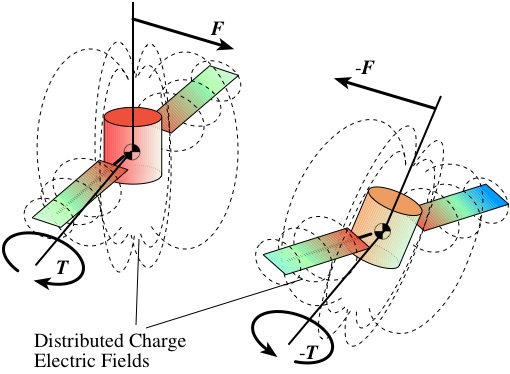
\includegraphics[width=3.5in]{Figures/test}
%	\caption{Illustration Caption Goes Here}
%	\label{fig:xxx}
%\end{figure}
%
%\subsubsection{Figures.}   
%Illustrations are referenced by name and without formatting embellishments, such as Figure~\ref{fig:xxx}, Figure 2, \emph{etc}., or, Figures 3 and 4 (\emph{e.g}., not figure (1), Fig. 1, \underline{Figure 1}, \emph{Figure 1}, \emph{etc}.). Each illustration should have a caption unless it is a mere sketch. Single-phrase captions are usually in title case; they are bold 10-point serif font and centered below the figure as shown in Figure~\ref{fig:xxx}. An explanatory caption of several sentences is permissible. Ideally, every illustration should be legibly sized -- usually about one-half or one-quarter page -- and appear in the text just before it is called out or mentioned. Alternatively, it is also permissible to place all figures together at the end of the text as a separate appendix; however, these two conventions should not be mixed. All figures and callouts should remain clearly legible after reduction. All illustrations appear as black and white in the final printing, although colors are retained in the electronic (CD-ROM) version.


%\subsubsection{Graphic Formats.} 
%The highest quality formats are Encapsulated PostScript (EPS) and PDF vector-graphic formats. These formats are recommended for all illustrations, unless they create document files that are excessively large. Specifically, you should change the graphic format or compress the image resolution whenever an illustrated page takes more than two seconds to render onscreen, or, whenever the total manuscript file size starts to approach 5 Mb. Photographs, illustrations that use heavy toner or ink (such as bar graphs), and figures without text callouts, may be suitably displayed with picture formats such as BMP, GIF, JPEG, PNG, TIFF, \emph{etc}. Line drawings, plots, and callouts on illustrations, should not use picture formats that do not provide sharp reproduction. All graphical content must be embedded when creating a PDF document, especially any fonts used within the illustration. Note that the Windows Metafile Format (WMF) is sometimes problematic and should be avoided.


%\subsubsection{References and Citations.} 
%The citation of bibliographical endnote references is indicated in the text by superscripted Arabic numerals, preferably at the end of a sentence.\cite{doe2005, style1959}   If this citation causes confusion in mathematics, or if a superscript is inappropriate for other reasons, this may be alternately expressed as (Reference~\citenum{doe2005}) or (see References~\citenum{doe2005} and \citenum{style1959}), (\emph{e.g}., not [1], Ref. (1), \emph{etc}.). While there is no singly prescribed format for every bibliographical endnote, references should be consistent in form. Citations should be sufficient to allow the reader to precisely find the information being cited, and should include specific pages, editions, and printing numbers where necessary. URL citations are discouraged, especially when an archival source for the same information is available. If a URL citation is required, it should appear completely and as a footnote instead of a bibliographical reference.\footnote{\url{http://www.univelt.com/FAQ.html\#SUBMISSION}}  The citation of private communication is especially discouraged, but if required it should be cited as a footnote and include the date, professional affiliation, and location of the person cited.\footnote{Gangster, Maurice (1999), personal correspondence of March 21st. Sr. Consultant, Space Cowboy Associates, Inc., Colorado Springs, CO.}  



%\begin{table}[htbp]
%	\fontsize{10}{10}\selectfont
%    \caption{A Caption Goes Here}
%   \label{tab:label}
%        \centering 
%   \begin{tabular}{c | r | r } % Column formatting, 
%      \hline 
%      Animal    & Description & Price (\$)\\
%      \hline 
%      Gnat      & per gram & 13.65 \\
%                & each     &  0.01 \\
%      Gnu       & stuffed  & 92.50 \\
%      Emu       & stuffed  & 33.33 \\
%      Armadillo & frozen   &  8.99 \\
%      \hline
%   \end{tabular}
%\end{table}

%\emph{Tables.} 
%Tables are referred to by name in the text as Table~\ref{tab:label}, or, Tables 2 and 3 (\emph{e.g}., not table 1, Tbl. 1, or \emph{Table 1}). The title is centered above the table, as shown in Table 1. The font size inside tables should be no larger than the body text, but may be adjusted down to 9-point if necessary (10-point serif font is considered nominal). Note that table units are in parentheses. Only the minimum number of table lines needed for clarity is desired. Ideally, every table should appear within the text just before it is called out, but, it is also permissible to place all tables together at the end of the text as a separate appendix. If so, these two conventions should not be mixed.
%
%Equations, figures, and tables must be sequentially numbered with no repeated numbers or gaps. Each figure and table shall be called out in the text; gratuitous figures and tables that are not called out should be eliminated. Intermediate equations may be numbered without being called out.






%Space-based surveillance can be highly effective at estimating foreign spacecraft or objects. Angles-only orbit determination is a visual sensing technique for relative orbit determination passively; i.e. light from a deputy satellite is captured by the chief, unlike a radar system wherein waves must be emitted from an external source.


